\documentclass[UTF8,a4paper,11pt,fontset=fandol]{ctexart}
\IfFontExistsTF{Droid Sans Fallback}
  {\newCJKfontfamily\cjkfallback{Droid Sans Fallback}}
  {\IfFontExistsTF{Noto Sans CJK SC}
    {\newCJKfontfamily\cjkfallback{Noto Sans CJK SC}}
    {\newcommand{\cjkfallback}{\CJKfamily{song}}}}
\usepackage[margin=22mm,headheight=15pt]{geometry}
\usepackage{graphicx,float,xcolor,amsmath,amssymb,booktabs,longtable,array,tabularx}
\usepackage[most]{tcolorbox}
\usepackage{listings,needspace,fancyhdr,enumitem}
\setlist{leftmargin=2em,itemsep=0.35em,topsep=0.4em,parsep=0pt}
\usepackage[unicode,colorlinks=true,linkcolor=blue!45!black,urlcolor=blue!45!black,breaklinks=true]{hyperref}
\usepackage{xurl}
\setlength{\parindent}{0pt}
\setlength{\parskip}{0.65em}
\setlength{\emergencystretch}{3em}
\linespread{1.14}
\raggedbottom
\pagestyle{fancy}\fancyhf{}\fancyhead[L]{月球大叔 · 访谈学习笔记}\fancyfoot[C]{\thepage}
\newtcolorbox{importantbox}[1]{enhanced,breakable,colback=blue!3,colframe=blue!45!black,title={#1},fonttitle=\bfseries}
\newtcolorbox{knowledgebox}[1]{enhanced,breakable,colback=teal!3,colframe=teal!50!black,title={#1},fonttitle=\bfseries}
\newtcolorbox{warningbox}[1]{enhanced,breakable,colback=orange!4,colframe=orange!60!black,title={#1},fonttitle=\bfseries}
\lstset{basicstyle=\ttfamily\small,breaklines=true,columns=fullflexible,keepspaces=true,showstringspaces=false,frame=single,captionpos=b}
\newcolumntype{Y}{>{\raggedright\arraybackslash}X}
\newcommand{\notetitle}{Brandon 陈春宇谈创业与产品：从反复尝试到跨语言沟通}
\newcommand{\videocoverpath}{cover.jpg}
\newcommand{\videourl}{https://www.youtube.com/watch?v=jjyG9-dNZAo}
\newcommand{\videochannel}{月球大叔}
\newcommand{\videopublishdate}{2026-10-23}
\newcommand{\noteauthors}{月球大叔、Brandon 陈春宇}
\newcommand{\sourceurl}{https://www.youtube.com/watch?v=jjyG9-dNZAo}
\begin{document}

\begin{titlepage}\centering\vspace*{4mm}
{\Large 月球大叔 · 访谈学习笔记\par}\vspace{8mm}
{\LARGE\bfseries \notetitle\par}\vspace{7mm}
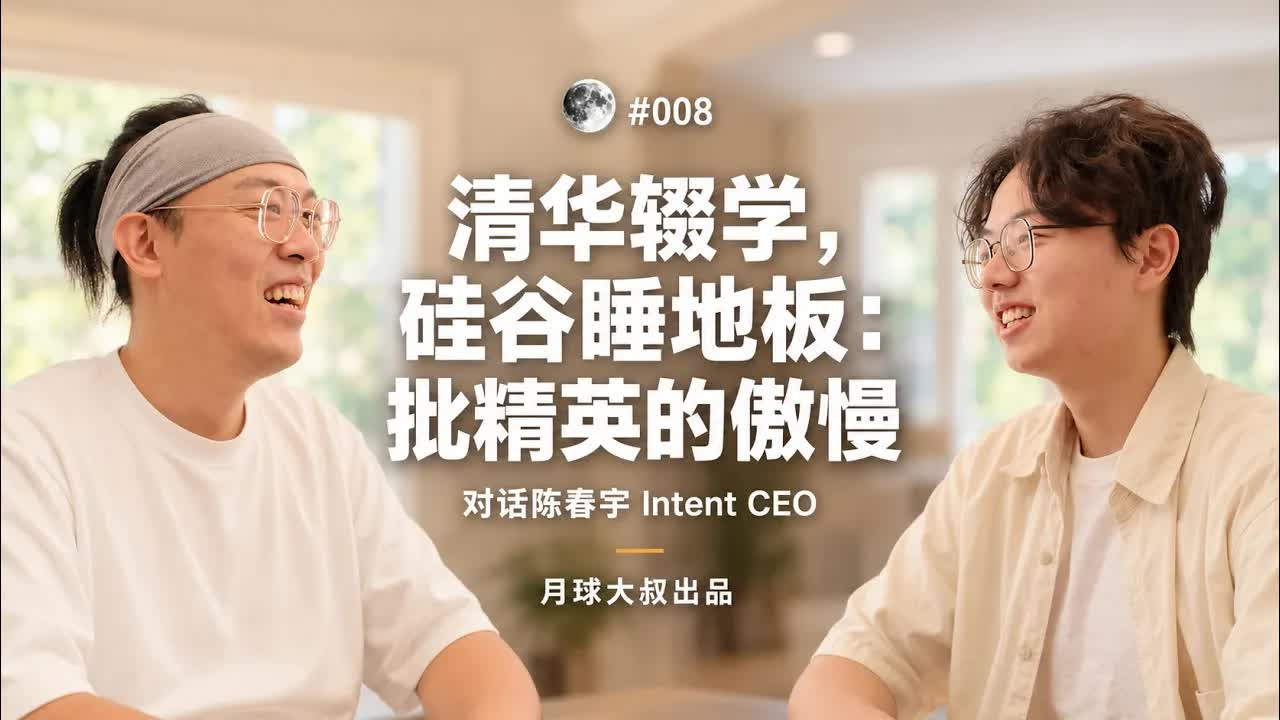
\includegraphics[width=.86\linewidth,height=.27\textheight,keepaspectratio]{cover.jpg}
\par\vspace{6mm}{\small 原节目：陈春宇: 清华，辍学，睡地板，精英的傲慢，硅谷，创业，情商，聊天软件，全球翻译，生物，爱自己\par}
\vspace{4mm}主播：月球大叔\par
{\small Brandon 陈春宇\par}
\vfill 发布：2026-10-23\par
整理：2026-10-25\quad 正文：Gemini Argon\quad 配图与编校：Codex\par
\vspace{4mm}\url{https://www.youtube.com/watch?v=jjyG9-dNZAo}
\end{titlepage}
\begingroup\small\setlength{\parskip}{0pt}\tableofcontents\endgroup\clearpage
\section*{导读}\addcontentsline{toc}{section}{导读}
这份技术与创业学习笔记整理自对极群科技及跨语言沟通应用Intent创始人陈春宇（Brandon）的深度访谈。笔记围绕他从高中进入大学实验室、本科期间离开校园初次创业，到2022年后在AI应用方向上反复试错并转向跨语言即时通讯产品的经历展开。全篇不试图提炼标准的成功公式，而是聚焦于三个可借鉴的实践层面：一是如何通过提前参与真实任务来观察自身兴趣与日常工作的适配度；二是如何在早期融资交割、大厂业务合作与多次产品原型迭代中，区分注册、留存、使用频次与真实付费等不同层次的证据；三是技术团队如何通过客户端工程实现、语音识别至语音合成（ASR—翻译—TTS）链路打磨及社区实地观察，理解不同语言用户的具体沟通处境。
\needspace{8\baselineskip}\section{先体验一种生活，再决定是否继续}
面对一条被许多同龄人向往的升学与职业路径，年轻人往往要在投入数年时间后才意识到自己是否适应那种日常工作状态。本章通过陈春宇在中学与本科阶段的早期探索经历，介绍他如何通过提前参与实验室工作来观察自身兴趣与科研日常的适配度，以及在调整方向时，如何借助学校制度与沟通方式减少摩擦，并反思过度迎合外界评价对个人表达欲的影响。
\needspace{6\baselineskip}\subsection{提前接触科研带来的判断}
许多学生在填报志愿或规划职业时，主要依赖学校声誉或学科印象来做决定，较少有机会提前了解该领域的日常工作状态。陈春宇在2017年通过第26届全国生物学竞赛第6名的成绩保送清华大学。由于在备战竞赛期间已经提前学完了大学本科甚至部分研究生的专业课程，他在高二暑假做了一个决定：主动联系清华大学生命科学学院的教授，申请进入实验室工作。在高三到大一期间，包括大学正式开学前，他自己来到北京打工赚取房租，在实验室里与博士生一起做实验，还在高中阶段带过\textbf{轮转博士生}（Rotation PhD student，指刚入学、需要在不同实验室短期工作以实现师生双向选择的博士生）。

这段实验室经历很快带来了学术成果。他在高三到大一期间参与的科研工作陆续发表了两篇论文，其中一篇发表在化学领域的知名期刊《德国应用化学》（Angewandte Chemie）上。然而，提前走完从实验操作到论文发表的流程，并没有让他留在学术界，反而促使他做出了转换方向的个人选择。

在陈春宇当时的个人感受里，这段经历让他提前看到了如果按部就班读完本科、博士再做博士后的生活状态：对他而言，那意味着将大一已经走通的发论文流程继续重复下去，把一篇文章变成五篇、十篇。在评估自身条件时，他将自己与张锋、庄小薇等顶尖华人生物学家对比，觉得自己并不具备那样突出的科研天赋，并发出“生物多我一个不多，少我一个不少”的感慨。既然已经知道自己能完成这类工作，又觉得自己在这一方向上缺少突出的长处或持续的热情，他便开始思考实验室之外的其他路径。

\needspace{6\baselineskip}\subsection{从一封邮件开始争取机会}
在许多同龄人看来，一个高中生能够进入清华实验室参与科研并不常见。按照常规印象，这类机会往往集中在人大附中、上海中学等一线城市知名中学的学生手中。但陈春宇来自江西上饶的上饶中学——一所四五线地级市的中学，也并非江西省内最顶尖的重点高中。主持人也提到，自己直到大三才意识到应该去找实验室体验博士生活。那么，在缺乏一线城市人脉的情况下，这种主动争取机会的想法和行动是从何而来的？

陈春宇将其归因于从小在宽松家庭教育中积累的正向激励。他回忆道，小学二三年级时，每天上学都要经过一条车流量很大、人车分流不合理的马路。父亲鼓励他：“如果你觉得这里应该建个天桥，就可以给市长信箱写封信。”他真的写了一封信，两年后那条马路上建起了一座天桥。陈春宇明确表示，自己并不知道天桥的建设与那封信之间是否存在任何关系，但对于一个小学生而言，这次尝试成了一次很强的正向激励，让他觉得遇到问题时主动表达是值得一试的。

到了初三和高中学竞赛的阶段，这种主动尝试的习惯被延续了下来。参加各类培训班时，他会主动找授课教授聊天、加微信并询问能否分享课件。虽然经常遭到拒绝，但他当时的感受是：只要成功一次，对自己来说就没有什么损失，还能获得正向反馈。带着这种心态，他觉得给清华教授发邮件是一件可以直接去做的事：打开学院官方网站，进入教师团队页面，查看每位老师的研究方向、代表性论文与公开邮箱，在认真读完论文后写邮件联系。当然，主动联系也需要投入阅读文献与沟通的时间成本，并非每次都能得到回应；但这种从公开渠道寻找切入点的具体做法，仍可整理为以下几个步骤：
\begin{itemize}
\item \textbf{检索公开渠道}：直接访问目标学院官网的教师名录，查看公开的研究方向、代表作与联系邮箱。
\item \textbf{前置功课准备}：在联系前认真阅读对方的代表性论文，让邮件内容建立在对实验室工作的具体了解之上。
\item \textbf{平和面对未回复或拒绝}：主动联系需要承担准备与沟通成本，也可能常遇拒绝，但认清这是正常现象后，便更容易迈出第一步。
\end{itemize}

\needspace{6\baselineskip}\subsection{休学、沟通与自己的选择}
当陈春宇在2021年接近大三时决定离开清华去创业，他面临的另一个现实问题是如何与父母及学校沟通。在常见的家庭与教育观念中，直接宣布“清华我不读了”很容易让家里陷入激烈争执。为此，他采取了“先开扇窗、再开扇门”的沟通方式，先向父母提出办理“休学”。他向父母说明，休学以后随时可以回校，而且这是一次很好的锻炼和学习机会；当时清华大学正好有创业休学政策，在他所述的那一政策下可休学三年，父母听说还能回校便同意了。作为一项正式的学籍管理制度，休学本身就为学生保留了回校继续学业的通道，客观上也为家庭沟通提供了缓冲。

这种先办休学的沟通方式在面对家人、当时的伴侣以及身边人时都减小了摩擦阻力。而当陈春宇拿着休学申请表，去找学院当时负责本科生工作的副院长并同样表示“先休学再说”时，副院长直接对他说：“你这个还回来干啥，别回来了。”这句话让陈春宇觉得说到了自己心里，因为他当时确实不想回来，只是为了减少与外界评价体系的碰撞，才对身边人反复表示还会回校。后来在访谈后段（01:47:33–01:49:14）回应“如何给想辍学创业的清华学弟学妹提建议”时，他也基于自己的经历谈道：关键是找到真正想做的事；如果学生时代感到被“GPA必须拿3.9”等条框束缚，在自己特别需要时间且有能力承担相应风险的前提下，可以考虑退课或利用学校当时的三年创业休学政策腾出时间。他还提到，如果因为答应了小组合作而不好意思退课，可以请同学吃饭并诚恳致歉说明情况；当然，涉及课程团队协作时，妥善沟通并处理好交接本就是应尽的责任。

不过，这种习惯用圆滑方式减小阻力的做法，也让陈春宇在后来产生了反思。在一次去一位企业家前辈家中唱卡拉OK时，对方提醒了他一句，让他开始思考自己这几年是不是“情商太高了”。陈春宇在访谈中用自己的话描述这种状态：当一个人过多思考别人的感受、在说每一句话前都在大脑里加上一层“审核机制”和“改写机制”以减小冲突时，他觉得自己会失去\textbf{利比多}（Libido，陈春宇在访谈中用这一概念来形容生命力、最原始想表达的东西与主体性）。他坦言，自己没有一上来就拿到彼得·蒂尔奖学金（Thiel Fellowship）直接进入硅谷核心圈的机会，正是靠着一定程度的妥协与圆滑，才一步步筹到赴美差旅费、办下美国工作签证并带着同伴做事；但他认为这也曾在一段时间内压抑了自己的长板与个性，让他没能在真正想做的事情上倾注全部心力。主持人在听完后也提到自己读博（PhD）期间经历不佳、艰难毕业时一位院长给他的建议：身处特定环境时，需要坚守本心并用一定手段保存自己、拿到想要的东西，直到脱离该环境。陈春宇就此总结道，需要分清目的和手段——圆滑可以作为需要时调用的一项技能，但不应反客为主，变成时刻影响思维方式的生命主旋律。

\begin{knowledgebox}{通过提前参与真实工作观察适配度}
在投入长周期的学业或职业轨道之前，仅凭课程成绩或外界印象往往难以判断自身是否适应那种日常状态。陈春宇的做法是在高二暑假至大一期间进入实验室，实际参与做实验、带轮转生与发表期刊论文的过程。这种提前体验有助于把抽象的职业名称转化为具体的日常感受，帮助个人观察两件事：一是自己对这类日常任务的持续性工作是否有热情；二是在了解真实工作内容后，评估自身兴趣、能力特点与该方向的适配程度，从而为继续深造或转向其他领域提供参考。
\end{knowledgebox}
\begin{importantbox}{陈春宇对“沟通手段”与“个人表达”的反思}
在做出离开校园等非常规选择时，利用学校既有的休学制度并采取温和的沟通方式，有助于减少与家庭及现有评价体系的摩擦，在特定阶段帮自己争取时间、差旅费或签证条件。但陈春宇根据自身经历提醒，如果把这种减小冲突的圆滑做法变成习惯，在每次表达前都对想法做一层自我审核与改写，他感到这会压抑自己的表达欲与主体性（他称之为“利比多”）。因此他主张把圆滑当作特定情境下的沟通技能，同时为自己寻找一个不被评判、能够直接说出真实想法的环境。
\end{importantbox}
\begin{table}[H]\centering\small
\caption{陈春宇早期探索中的三次具体行动与个人取舍}
\begin{tabular}{>{\raggedright\arraybackslash}p{\dimexpr(\linewidth-6\tabcolsep)/3\relax}>{\raggedright\arraybackslash}p{\dimexpr(\linewidth-6\tabcolsep)/3\relax}>{\raggedright\arraybackslash}p{\dimexpr(\linewidth-6\tabcolsep)/3\relax}}
\toprule
行动场景 & 解决的核心问题 & 具体机制与取舍权衡\\\midrule
高二暑假发邮件进清华实验室 & 如何打破信息差并验证自身是否适合长期科研 & 通过学院官网查看公开的研究方向、代表论文与邮箱并写信联系；虽需投入读论文时间且常遇拒绝，但成功进入实验室让他得以提前体会科研日常。\\[4pt]
以“创业休学”替代直接退学 & 如何在减小家庭与外界评价摩擦的前提下离开校园创业 & 采用“先开窗再开门”的沟通方式，借助当时学校可休三年的创业休学政策作为缓冲；减小了沟通阻力，但当时也感到难以对身边人直说不想回校的真实想法。\\[4pt]
反思“高情商”与大脑审核机制 & 如何在争取现实资源的同时避免丧失创造力与主体性 & 认为圆滑曾帮自己筹措赴美路费和签证，但也感到过度自我审核压抑了个性与长板；希望将其限制为按需使用的技能而非思维习惯。\\[4pt]
\bottomrule\end{tabular}\end{table}
年轻人在规划学业与职业时，往往只能凭外界印象做决定，很难提前知道自己是否适应那种日常状态。陈春宇在高二暑假至大一期间进入清华实验室的经历，展示了一条通过提前参与真实任务来辅助判断的路径。
\begin{figure}[H]\centering
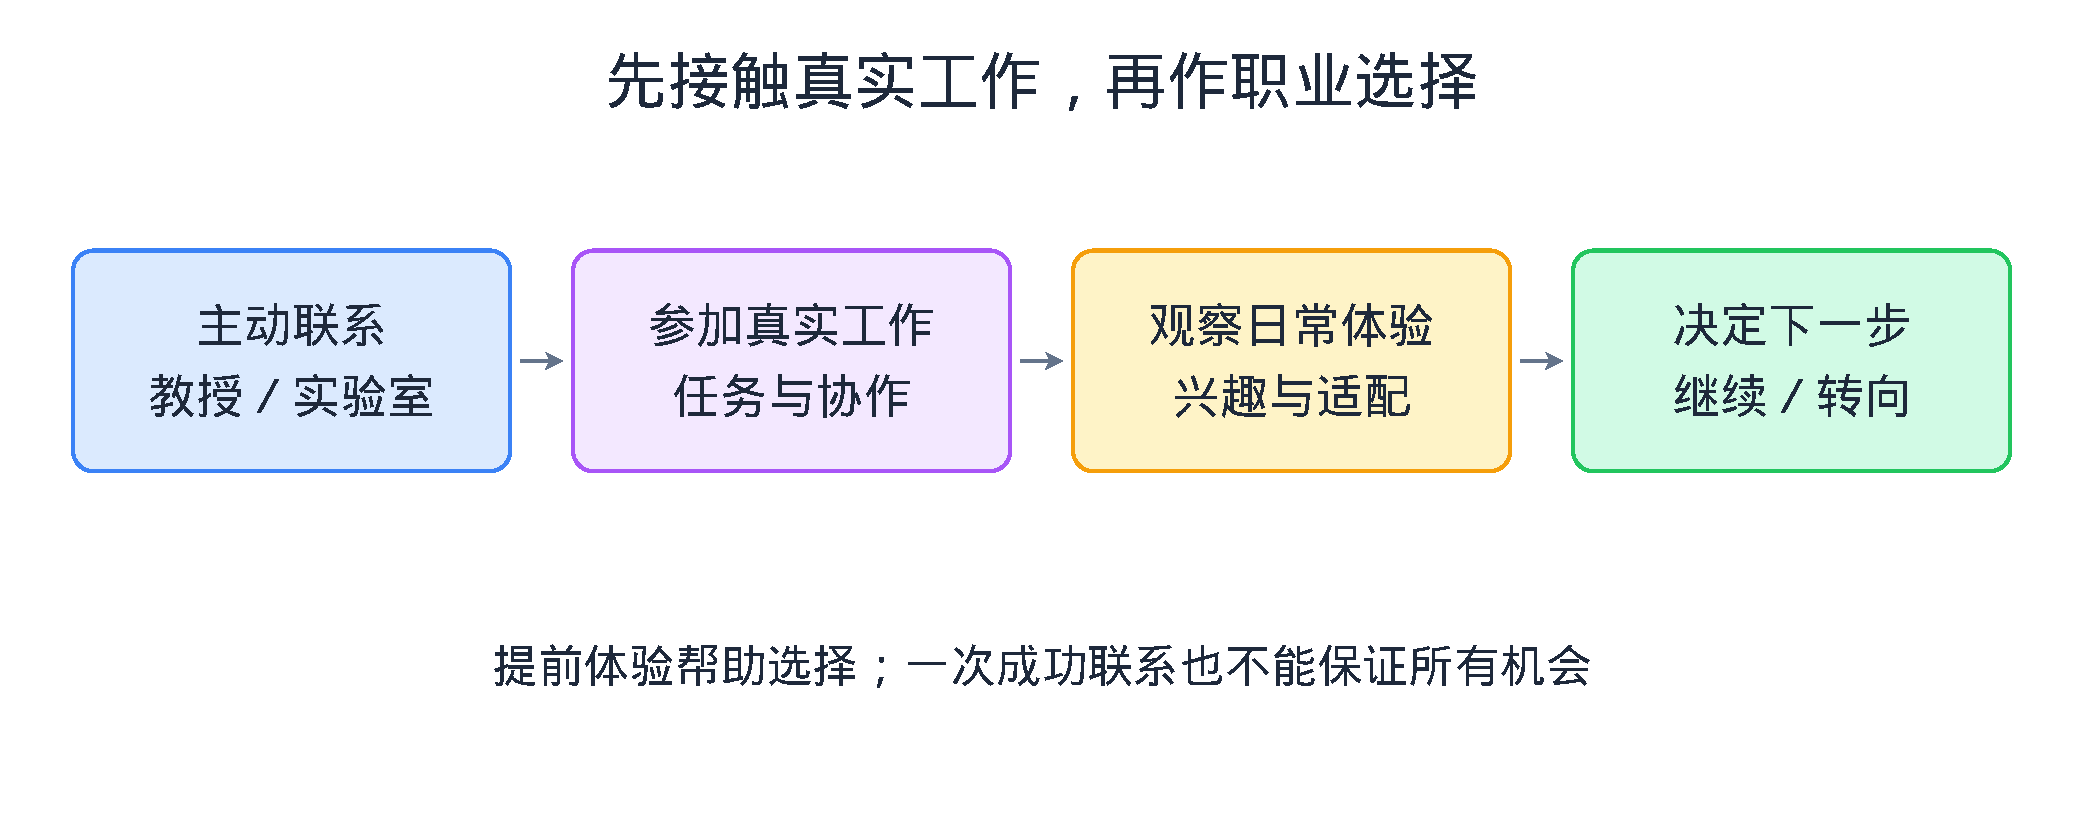
\includegraphics[width=\linewidth,height=.68\textheight,keepaspectratio]{assets/early-experience.pdf}
\caption{先接触真实工作，再作职业选择；依据访谈00:00:37–00:12:07口述整理}
\end{figure}
\begin{knowledgebox}{读图：先体验一种生活，再决定是否继续}
本图上方由四个从左到右以箭头相连的圆角矩形组成：第一步是蓝色框“主动联系：教授／实验室”，指向第二步紫色框“参加真实工作：任务与协作”，再指向第三步黄色框“观察日常体验：兴趣与适配”，最后指向第四步绿色框“决定下一步：继续／转向”。图下方有一行居中文字提醒：“提前体验帮助选择；一次成功联系也不能保证所有机会”。
\end{knowledgebox}
这种提前接触真实工作的做法，重点在于观察自身对具体日常任务的兴趣与适配度；而在做出转向创业的决定后，如何在首家公司里面对商业与融资规则，则是下一章探讨的问题。
\needspace{6\baselineskip}\subsection{本章小结}
\begin{itemize}
\item \textbf{提前接触真实工作辅助判断}：通过尽早进入实验室参与具体实验和论文写作，陈春宇根据自身对日常工作重复度的感受与能力评估，做出了不再继续走十年学术路径的个人决定。
\item \textbf{借助公开信息主动联系}：在缺乏一线城市名校人脉时，通过学院官网阅读代表作并发邮件联系老师；认清被拒是常见情况并愿意承担沟通成本，有助于争取到实际的参与机会。
\item \textbf{善用制度缓冲并分清手段与目的}：面对家庭与学校环境，可借助休学等正式制度减小沟通阻力；同时留意避免让迎合外界评价的“自我审核”成为日常思维习惯。
\end{itemize}
\needspace{8\baselineskip}\section{第一家公司教会了什么}
提前结束实验室工作后，陈春宇在大二陷入了对未来出路的迷茫。本章顺着他2021年前后的经历，看他的生物竞赛与社团活动背景如何与当时的行业招聘需求交会，并复盘他从校园游戏社团走向第一家创业公司时，在融资意向、交割推进与个人退出上经历的具体教训。
\needspace{6\baselineskip}\subsection{职业热潮与个人经历的交会}
当大一就把实验室的科研工作基本做完后，陈春宇在大二感到十分迷茫。他当时觉得生物专业的出路似乎只有当竞赛教练、高中老师，或者去\textbf{CRO}（合同研究组织，为医药企业提供外包研发服务的机构）做实验技术员。看到金融行业的高薪，他甚至后悔当年凭借国赛名次没有选择北大元培学院再走光华管理学院方向，去争取中金、中信或风险投资机构的实习。陈春宇在访谈中将当时的心境与现在一些年轻人的想法作类比：就像现在不少朋友会想“进不了\textbf{Frontier Labs}（前沿大模型实验室）人生是不是就完蛋了”一样，每个时期都有人们眼中的热门路径，一旦觉得自己没赶上，就容易陷入焦虑与自我怀疑。

转机出现在2021年。当时国内合成生物学投资升温，投资机构需要能看懂生物医药与合成生物学的实习生。陈春宇此前曾担任清华大学\textbf{iGEM}（国际基因工程机器大赛）队长之一，带队赴波士顿MIT参赛并取得了当时清华的历史最佳成绩与两个单项奖。在2021年这一特定招聘窗口下，这段经历正好契合了机构的需要——当经管背景的大二、大三学生较难迅速看懂合成生物学时，他在找实习网站上投递了第一页的几家公司，十余分钟后便接到HR电话。一位清华学长专门打车到校门口面试他，带他进入了\textbf{VC}（风险投资机构）源码资本实习，几乎同一时间他还接到了摩根士丹利旗下二级市场基金的面试电话。

陈春宇回忆起当时一个有些狼狈的插曲：他在简历上声称自己会看财务报表，实际上却完全不会。入职第二三天就需要看表时，在那个还没有ChatGPT可以随时提问的年代，他只能连夜找书恶补资产负债表、利润表和现金流量表这“财务三张表”，边学边写投资\textbf{Memo}（投资备忘录，用于内部梳理项目情况的评估文档）。因为比同届生物系同学更早完成了实验室阶段的工作，他得以更早出来探索，随后还拉了微信群，帮不少“生化环材”背景的同学修改简历、内推金融实习。在与主持人交流这段经历时，他感慨不同专业背景能否刚好遇上行业需求，很大程度上要看行业周期能不能与个人20岁到30岁的起步阶段对上，因此也需要根据实际情况主动调整方向。

\needspace{6\baselineskip}\subsection{从校园游戏社区开始创业}
由于早早修完了专业课，大三的陈春宇没有把全部精力用来刷题卷实习，而是留出时间在校园里折腾感兴趣的事。当时他在清华大学“次世代动漫社”的大群里，响应同学号召一起搭建了清华运营时间最长、最活跃的\textbf{Minecraft}（《我的世界》，一款高自由度的沙盒建造游戏）服务器，并成为第一批管理员。管服过程中，发起服务器的搭档提议：“要不我们自己做个游戏吧？”这次略带玩票性质的提议，直接开启了他的第一段创业经历。

两人随后报名参加清华大学“校长杯”创业大赛。到了预审现场，他们发现周围全是实验室硬科技成果转化项目，自己显得格格不入，甚至在初赛阶段就被老师劝退。有趣的是，当时他和搭档都还在VC实习，参赛原本还抱有一点潜入创业选手群帮机构物色项目的心理。结果路演当天陈春宇在外地出差，担任CEO的一号位搭档独自去现场，下午突然打来电话说有投资人看中了他们，约晚上去瑰丽酒店见合伙人。

那天晚上在酒店里，两个年轻人其实连具体要做什么都还讲不清楚，只是模糊地提出想做游戏创作平台、游戏UGC（用户生成内容），以及比\textbf{Unity}和\textbf{Unreal Engine}（虚幻引擎，Epic Games旗下的游戏开发引擎）更好的游戏创作工具。当投资人问做出这个工具需要多少钱时，两人并不了解工业级游戏引擎的研发规模——搭档原本想报100万人民币，为了留出砍价空间便随口报了120万人民币。没想到对方没有砍价，直接表示愿意投资。陈春宇坦言，这笔120万只是当时为了留砍价空间报出的数字，并非经过测算的开发预算；那完全是“无知者无畏”，直到投资人表示要投之后，连Unity和Unreal都没怎么用过的他们，才去买了一本叫《游戏引擎》的书开始研读。

\needspace{6\baselineskip}\subsection{投资意向、交割和退出}
瑰丽酒店的那位投资人随后带着他们去国贸酒店见了知名投资人朱啸虎。陈春宇和搭档与朱啸虎聊了约十分钟，对方当场口头表示愿意出资600万人民币（按当时汇率约合100万美元）占股10\%。然而，陈春宇明确提到，他们最终并没有拿到朱啸虎的这笔钱。由于团队当时毫无融资经验，在后续推进\textbf{SPA}（股份购买协议）和\textbf{SHA}（股东协议）等法律文件时拖拖拉拉，据他事后回顾，当时在一些不太重要的细节上耗费了不少时间。等投资人的兴头过去，这笔投资意向便被撤回（drop）了；过了几年陈春宇才听说，当时对方对他们的评价是“团队太作”。这次挫折让他和主持人共同总结出早期融资的一条经验：口头投资意向并不等于资金到账，创业者需要理解\textbf{Close}（交割，即完成最终协议签署、满足约定条件且资金实际打入公司账户）的重要性。

在这笔意向告吹之后，另一家早期投资机构的实习生在LinkedIn上加上了陈春宇，来办公室考察后带他们去见了机构合伙人，对方当场给出了\textbf{TS}（Term Sheet，投资条款清单）。陈春宇回忆，因为此前经历过一次投资被撤回，他们这次拿到TS后没有再纠结估值和条款细节，当场签了字，并在随后的流程中实际拿到了约100万美元（约合六七百万人民币）的融资。需要注意的是，在商业实践中，TS通常用于明确投资的核心框架（其中保密、排他等条款可能具有相应约束力），签下TS仍不等于完成最终交割；而陈春宇当时“不管条款直接签字”只是他受前次挫折影响下的个人反应，在实际交易中仍应审慎理解协议内容并落实交割条件。

然而，这家公司在拿到钱后不到一年便停止了运转。在第一轮与第二轮资金衔接的困难时期，陈春宇和担任CEO的一号位搭档曾自己掏钱垫付公司运营资金，一起租住在清华校外的华清家园没日没夜地干活。事后陈春宇反思，当时只有20岁的他们还没有想清楚成为创业者意味着什么，在没经历过太多磨难的情况下相对容易地拿到了资金，后续的成长速度却没能跟上；就他个人而言，他对这个方向缺乏足够的\textbf{Conviction}（坚定的信念感），当时也还没有学会如何面对长期没有正反馈的过程。

发觉自己信念感不足后，陈春宇比公司最终结束更早一步向团队提出了退出。当时公司正在筹备搭建海外架构，他认为设立与后续维护海外架构需要额外开销，为了不给团队增加负担，便主动表示放弃全部个人股份，不需要为自己设立\textbf{BVI架构}（在英属维尔京群岛注册的离岸控股公司，常用于海外融资持股），在团队为他办了一场欢送会后直接离开；此后CEO与团队又继续尝试了一段时间，公司才最终画上句号。离开时，陈春宇还拿着自己做生物竞赛培训攒下的钱，主动找两位投资人沟通，提出愿意用现金赔付自己那部分股份对应的款项，两位投资人则体面地婉拒了。回看国贸酒店见到知名投资人的那个夜晚，陈春宇觉得，从决定走出校园接触这些人和事的那一刻起，自己学到的东西就已经很有收获。

\begin{importantbox}{早期融资中的意向、条款与交割}
在初次创业融资时，陈春宇团队曾将投资人的口头表态当作已经稳妥的融资，在后续推进SPA（股份购买协议）和SHA（股东协议）时拖延了进度，最终未能拿到那600万人民币。理解早期融资需要区分不同阶段：
\begin{itemize}
\item \textbf{口头意向}：投资人基于初步交流表达投资意愿，尚未形成书面文件，可能随时间或情况变化而终止。
\item \textbf{TS（投资条款清单）}：双方就估值、投资额与主要权利义务梳理出框架文件（部分条款如保密、排他可能具约束力），但签署TS仍不等于完成交割。
\item \textbf{正式协议与Close（交割）}：双方签署SPA、SHA等最终交易文件，落实交割条件，且投资款实际汇入公司账户。只有资金实际到账，才能真正用于公司运营。
\end{itemize}
\end{importantbox}
\begin{knowledgebox}{特定行业窗口下的跨专业求职案例}
陈春宇在2021年的求职经历，展示了个人过往投入如何与特定时期的行业招聘需求交会：他在本科期间因兴趣投入iGEM竞赛并带队获奖，恰好遇上2021年国内合成生物学一级市场投资升温，投资机构需要能看懂生物技术的实习生，这段经历便帮他获得了面试机会。至于他在简历中谎称会看财务报表、入职后才连夜看书补课的做法，属于他当时慌乱应付的插曲，求职与工作中仍应如实陈述技能并在岗位上扎实学习。
\end{knowledgebox}
\begin{table}[H]\centering\small
\caption{初次创业不同融资接洽阶段的表现与得失}
\begin{tabular}{>{\raggedright\arraybackslash}p{\dimexpr(\linewidth-6\tabcolsep)/3\relax}>{\raggedright\arraybackslash}p{\dimexpr(\linewidth-6\tabcolsep)/3\relax}>{\raggedright\arraybackslash}p{\dimexpr(\linewidth-6\tabcolsep)/3\relax}}
\toprule
接洽阶段与对象 & 解决的问题 & 机制与取舍\\\midrule
瑰丽酒店初见投资人 & 从校园Minecraft社团转向商业化立项，验证初步融资可能。 & 尚不了解工业级引擎研发规模，为留砍价空间报出120万人民币；获投资意向后才买《游戏引擎》研读。\\[4pt]
国贸见朱啸虎（10分钟） & 争取600万人民币（约100万美元）的知名机构早期资金。 & 获口头意向后，据其回顾在SPA/SHA条款推进中拖拉，未及时推进交割（Close），最终该笔投资未落地。\\[4pt]
LinkedIn机构实习生引荐 & 快速锁定约100万美元的实际早期启动资金。 & 受前次意向撤回影响，拿到TS后当场签字，后续实际获得约100万美元融资。\\[4pt]
项目后期个人退出 & 在个人信念感（Conviction）不足时先于公司结束退出团队 & 主动放弃个人股份、不设个人BVI架构，并提出用个人培训收入向投资人赔付（被婉拒）；团队此后又尝试了一段时间方才结束。\\[4pt]
\bottomrule\end{tabular}\end{table}
初次创业的年轻团队在接触风险投资机构时，容易把投资人当场的口头表态当作已经稳妥的融资。结合陈春宇第一家公司的经历，有必要将早期融资从初步意向到资金落地的不同阶段拆解清楚。
\begin{figure}[H]\centering
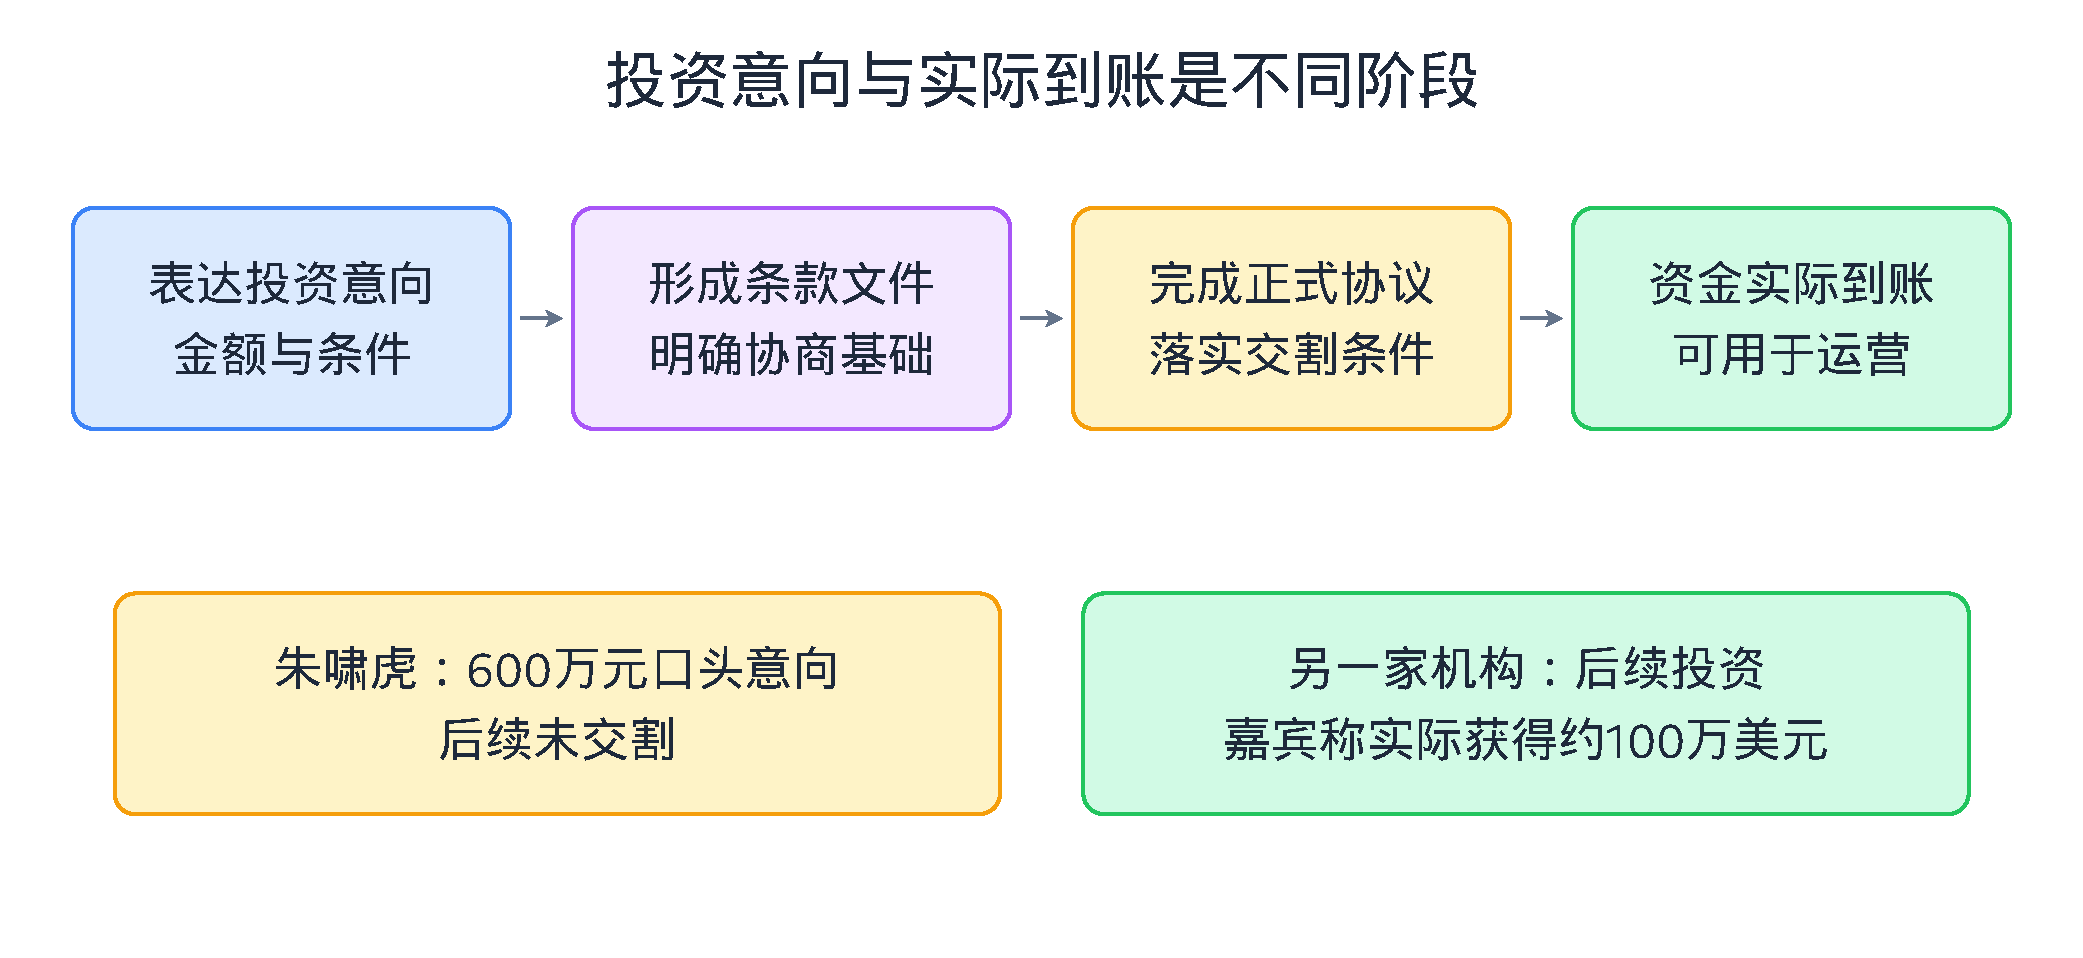
\includegraphics[width=\linewidth,height=.68\textheight,keepaspectratio]{assets/fundraising-stages.pdf}
\caption{投资意向与实际到账是不同阶段；依据访谈00:18:29–00:27:09口述整理}
\end{figure}
\begin{knowledgebox}{读图：第一家公司教会了什么}
本图分为上下两层。上层从左到右由四个以箭头依次连接的方框展示融资推进阶段：蓝色框“表达投资意向：金额与条件”指向紫色框“形成条款文件：明确协商基础”，再指向黄色框“完成正式协议：落实交割条件”，最终指向绿色框“资金实际到账：可用于运营”。下层左右并列两个对照框：左侧黄色框写着“朱啸虎：600万元口头意向／后续未交割”，右侧绿色框写着“另一家机构：后续投资／嘉宾称实际获得约100万美元”。
\end{knowledgebox}
分清口头意向、条款文件、正式协议与实际到账的区别，能帮早期团队避免将初步兴趣误判为可用资金；而当陈春宇离开首家公司、在2022年秋转向聊天机器人创业时，他又遇到了技术デモ如何进入真实业务的新考题。
\needspace{6\baselineskip}\subsection{本章小结}
\begin{itemize}
\item \textbf{留意专业经历与行业需求交会的窗口}：不必因未走上单一的热门路径而过度焦虑，陳春宇在iGEM竞赛上的投入恰好遇上2021年合成生物投资升温，帮他获得了进入VC实习的机会。
\item \textbf{区分口头意向、TS与实际交割（Close）}：朱啸虎的600万人民币口头意向最终未交割，而后续另一家机构的投资才实际到账；融资过程需分清意向、条款文件、正式协议与资金到账的不同阶段。
\item \textbf{坦诚面对信念感与团队去留}：当发觉自身对方向缺乏长期信念感（Conviction）时，陈春宇选择先于公司结束与团队沟通退出、放弃个人股份并主动向投资人交代，妥善处理了合作关系。
\end{itemize}
\needspace{8\baselineskip}\section{聊天机器人怎样走进真实业务}
从第一家游戏公司退出后，陈春宇继续留在自己熟悉的线上社群中观察。2022年秋，大语言模型公开前夕，他从日常聊天软件里的机器人权限问题切入，开启第二次创业。本章梳理他如何从群聊小工具起步，认识玩具代码与可用产品的距离，并在与百度等大厂及硅谷前辈的交流中，体会初创团队与成熟业务体系在创新方式上的差异。
\needspace{6\baselineskip}\subsection{让机器人参与聊天}
在离开第一家创业公司后，陈春宇于\textbf{2022年9月}创办了极群科技。这个切入点源于他本科期间常在QQ群、微信群以及海外即时通讯软件Telegram和Discord上活动的观察。当时大语言模型尚未普及，群聊里已经存在许多被称为\textbf{Bot（聊天机器人）}的自动化程序，它们大多依靠预设的关键词匹配来执行简单指令。按陈春宇在2022年前后的使用经验，主流社交平台对这些程序有着不同程度的限制：当时国内的QQ和微信对非官方机器人管控很严，账号容易被封禁；而在国外对机器人相对开放的Telegram和Discord上，他感到Bot依然处于类似“二等公民”的位置——例如在他当时的观察里，Bot与Bot之间无法直接对话，收发消息的权限也比真人账号低一等。这让他产生了一个初步想法：如果给程序赋予与真人用户相同的权限，让它像普通人一样活在群聊里，就能做许多事情。

围绕“给程序更多权限”的想法，由于当时同样不清楚该如何从头搭建新平台，团队决定先从群聊机器人做起。在ChatGPT公开前夕，他们一面尝试用传统的\textbf{NLP（自然语言处理，即计算机解析与处理人类语言的技术）}去做情感判断和模糊意图处理，一面接入了早期的开源图像生成模型\textbf{Stable Diffusion}，开发了一款群聊“你画我猜”Bot。因为当时的AI画图还不成熟，生成的图像往往相当诡异、让人摸不着头脑，这种不完美反而成了群友竞相猜测的乐趣。配合“成语接龙”“积功德”等群聊互动功能，这些小工具积累了几千名用户。不久后，陈春宇在一位清华学长（也是ChatGPT作者之一）的朋友圈里看到对方分享说组里做了一个小工作、欢迎大家体验，点进链接试用后深感震撼，意识到技术变革的齿轮已经开始转动。

\needspace{6\baselineskip}\subsection{从有趣的代码到可用的产品}
当主持人将这段在2022年秋天探索NLP与Bot的经历，与早期移动互联网创业者季逸超（Peak）以及硅谷早期的LangChain（大模型应用开发框架）等团队相提并论，认为他们“早早理解和布局了Agent（智能体）时代”时，陈春宇当场做出了坦诚的纠正。他指出，当时的自己完全谈不上理解与布局，甚至不知道什么是AI或Agent叙事；当同期的硅谷年轻创业者在YC（Y Combinator，硅谷知名创业孵化器）等机构的帮助下，已经在学习如何构建“人们真正需要的产品（build something people want）”、如何向风险投资人梳理叙事并融资时，他们还停留在校园独立开发者或小黑客（Hacker）的状态。把一段玩具级的代码写出来、让身边几百上千个同学在群里玩过之后，团队既不知道下一步该如何把玩具做成真正的产品，也受限于当时的英语水平和国内外互联网生态的差异，还不懂得如何在GitHub或海外社区展示作品。

尽管当时在能力、眼界和见识上受到限制，这段折腾依然让他保留了一条切身体会：\textbf{相信作为日常软件使用者和开发者的直觉，并认同“构建（build）的意义就在于构建本身”}。陈春宇认为，经常使用各类软件、查看API（应用程序编程接口）和开发者接口的人，所产生的直觉和感受并不比顶级风投机构（如a16z、Sequoia或YC）所投项目的创始人差。哪怕同样的想法别人能迅速拿到一千万美元种子轮，而自己还在为北京下个月的房租发愁，如果有动手构建的意愿，依然可以去做——不是为了迎合热门词汇（Buzzword）或在社交网络上制造踏空焦虑（FOMO），而是为了构建本身。当然，开发者的直觉仍需在后续的产品化与市场反馈中持续检验，他自己也坦言当时因为没有“年少有为”，所以用黄仁勋早年也当过洗碗工的传记故事来勉励自己不必过于着急。

\needspace{6\baselineskip}\subsection{与大厂合作需要理解业务}
让这群年轻开发者接触到大型企业业务的，是他们在奇绩创坛（由陆奇博士创办的早期创业孵化器）Demo Day（路演日）上的演示。当时，百度的人在路演上看到了他们的演示，随后找到团队并很快带他们见到了比李彦宏低一级别的资深副总裁，百度也由此成为极群科技的第一个客户。然而，双方在做了一些小项目后，合作并未能维系下去。面对主持人“是不是因为给企业客户做项目很容易变成外包、无法按自己意愿表达产品”的提问，陈春宇给出了明确的纠正。他表示，百度当时其实给了很大的宽容空间，希望他们能提出新想法来帮助把产品做得更好；合作未能持续的原因，在于团队当时对互联网业务与客户需求理解不足，也缺乏持续交付能力，暴露出\textbf{初创团队与成熟互联网公司在创新方式上的差异}。

陈春宇具体复盘了当时的处境：初创公司之所以能做出一些新尝试，往往是因为没有历史业务包袱，习惯在一张白纸上从头构想；而大型互联网公司在成熟业务上的创新，则建立在对自身产品生态、大量业务数据以及既有用户场景的深入理解之上。当他们这样一个对大厂业务生态理解不够、工程交付能力尚弱的早期小团队，试图在一个已经成熟的业务体系上做创新时，即便获得了高层的支持，实际能够调动的权限和资源整体上依然比较有限，结果发现无从下手。两边在尝试了几个方案（Proposal）且均未得到良好验证后，都觉得这种合作难以持续，陈春宇也借此认识到自己更想做的还是自己的产品。

在奇绩创坛期间，陈春宇为了给项目争取机会，非常主动地与导师陆奇博士保持沟通：他不仅把一对一交流（Office Hour）约满、在嘉宾讲座时占第一排挨着陆奇的位置坐，有一次为了汇报与百度的合作进展，甚至等在奇绩创坛的洗手间门口，趁陆奇洗手的间隙做了简短汇报（这类打扰他人私人空间的方式并不值得效仿，但反映了他当时急于争取指导的心态）。因为他在做聊天相关的方向，而Zoom当时恰好也想了解年轻人在聊天与机器人领域的想法，陆奇后来帮他引荐了Zoom创始人袁征（Eric Yuan）。\textbf{2023年6月}，陈春宇借这一契机飞往美国，在Zoom大楼里见到了袁征。当时他们还在讲述群聊多智能体（Multi-Agent）的想法，由于表达和故事梳理还不够清晰，方案被袁征评价为“感觉最后就是个Discord的Bot”，双方还交流了Discord在外界看不到的商业化考量。虽然这次会面没有成功获得投资，但能见到顶尖华人创业者依然给了他很大激励。到了后来的\textbf{2024年}，当他开始准备美国工作签证、产品在斯坦福大学上线推广时，因为没有SSN（美国社会安全号码，租房信用审查的常用凭证）很难租房，他和联合创始人便找了一位斯坦福大学的朋友，借住在对方宿舍地上的床垫上继续推进产品。

\begin{knowledgebox}{社交平台机器人（Bot）与智能体（Agent）应用}
智能体（Agent）本身是人工智能与计算机科学中早已存在的概念，强调程序能够感知环境并采取行动。而在2022年底大语言模型普及前，日常聊天软件里的\textbf{Bot（聊天机器人）}大多只能依靠预设规则、关键词匹配或传统自然语言处理（NLP）接口执行简单指令；在陈春宇当时的使用经验中，这类Bot还常受到平台权限限制（如无法直接互聊、收发消息权限低于真人账号）。随着大语言模型在上下文理解与文本生成能力上的提升，开发者得以让程序在群聊和应用中处理更复杂的模糊意图与互动任务。陈春宇团队的早期尝试，正是从观察聊天软件里的Bot权限限制出发，在大模型出现后转向探索群聊中的多智能体交互。
\end{knowledgebox}
\begin{importantbox}{陈春宇对大厂业务合作中断的复盘}
针对早期团队与百度合作未能延续的原因，陈春宇纠正了“大厂把小团队当外包”的猜测，从自身经历出发对比了两种不同的创新条件：
\begin{itemize}
\item \textbf{初创团队的从零尝试}：较少受既有产品形态的历史包袱限制，适合从头搭建新原型，但早期往往缺乏深厚的行业业务认知与稳定的持续交付能力（同时仍需面对资金与客户需求等现实约束）。
\item \textbf{成熟业务体系内的创新}：依赖对既有产品生态、业务数据和存量用户场景的深入理解；当外部小团队业务理解不足且实际可调动的权限、资源有限时，往往难以在成熟体系内做出有效验证。
\end{itemize}
\end{importantbox}
\begin{table}[H]\centering\small
\caption{极群科技早期探索阶段的认知与外部反馈对照}
\begin{tabular}{>{\raggedright\arraybackslash}p{\dimexpr(\linewidth-6\tabcolsep)/3\relax}>{\raggedright\arraybackslash}p{\dimexpr(\linewidth-6\tabcolsep)/3\relax}>{\raggedright\arraybackslash}p{\dimexpr(\linewidth-6\tabcolsep)/3\relax}}
\toprule
探索阶段与场景 & 试图解决的问题 & 实际机制与经验教训\\\midrule
群聊娱乐Bot（你画我猜、成语接龙） & 打破社交平台对程序的权限限制，让机器人在群里与人高频互动 & 利用早期Stable Diffusion画图怪异的特点做成猜图小游戏，积累几千名用户，但仍属玩具级代码，尚不清楚下一步如何产品化\\[4pt]
奇绩创坛Demo Day与百度合作 & 为早期AI互动技术寻找商业落地场景与大客户收入支撑 & 路演后获百度接触并见到资深副总裁，对方给予空间希望提新想法，但团队缺乏大厂业务生态理解与持续交付能力，几个方案均未跑通\\[4pt]
2023年6月赴美拜访Zoom创始人袁征 & 借陆奇博士引荐展示群聊Multi-Agent构想，寻求行业前辈指导与机会 & 因表达与叙事尚不成熟，方案被评价为类似Discord Bot；虽未获投资，但打通了赴美交流与实地试错的路径\\[4pt]
\bottomrule\end{tabular}\end{table}
在2022年秋创办极群科技时，陈春宇从聊天软件对机器人的权限限制切入，做出了几千名用户参与的群聊互动Bot，并在路演后接触到百度。但这引出了一个现实问题：有趣的机器人演示如何才能走进成熟的商业业务？
\begin{figure}[H]\centering
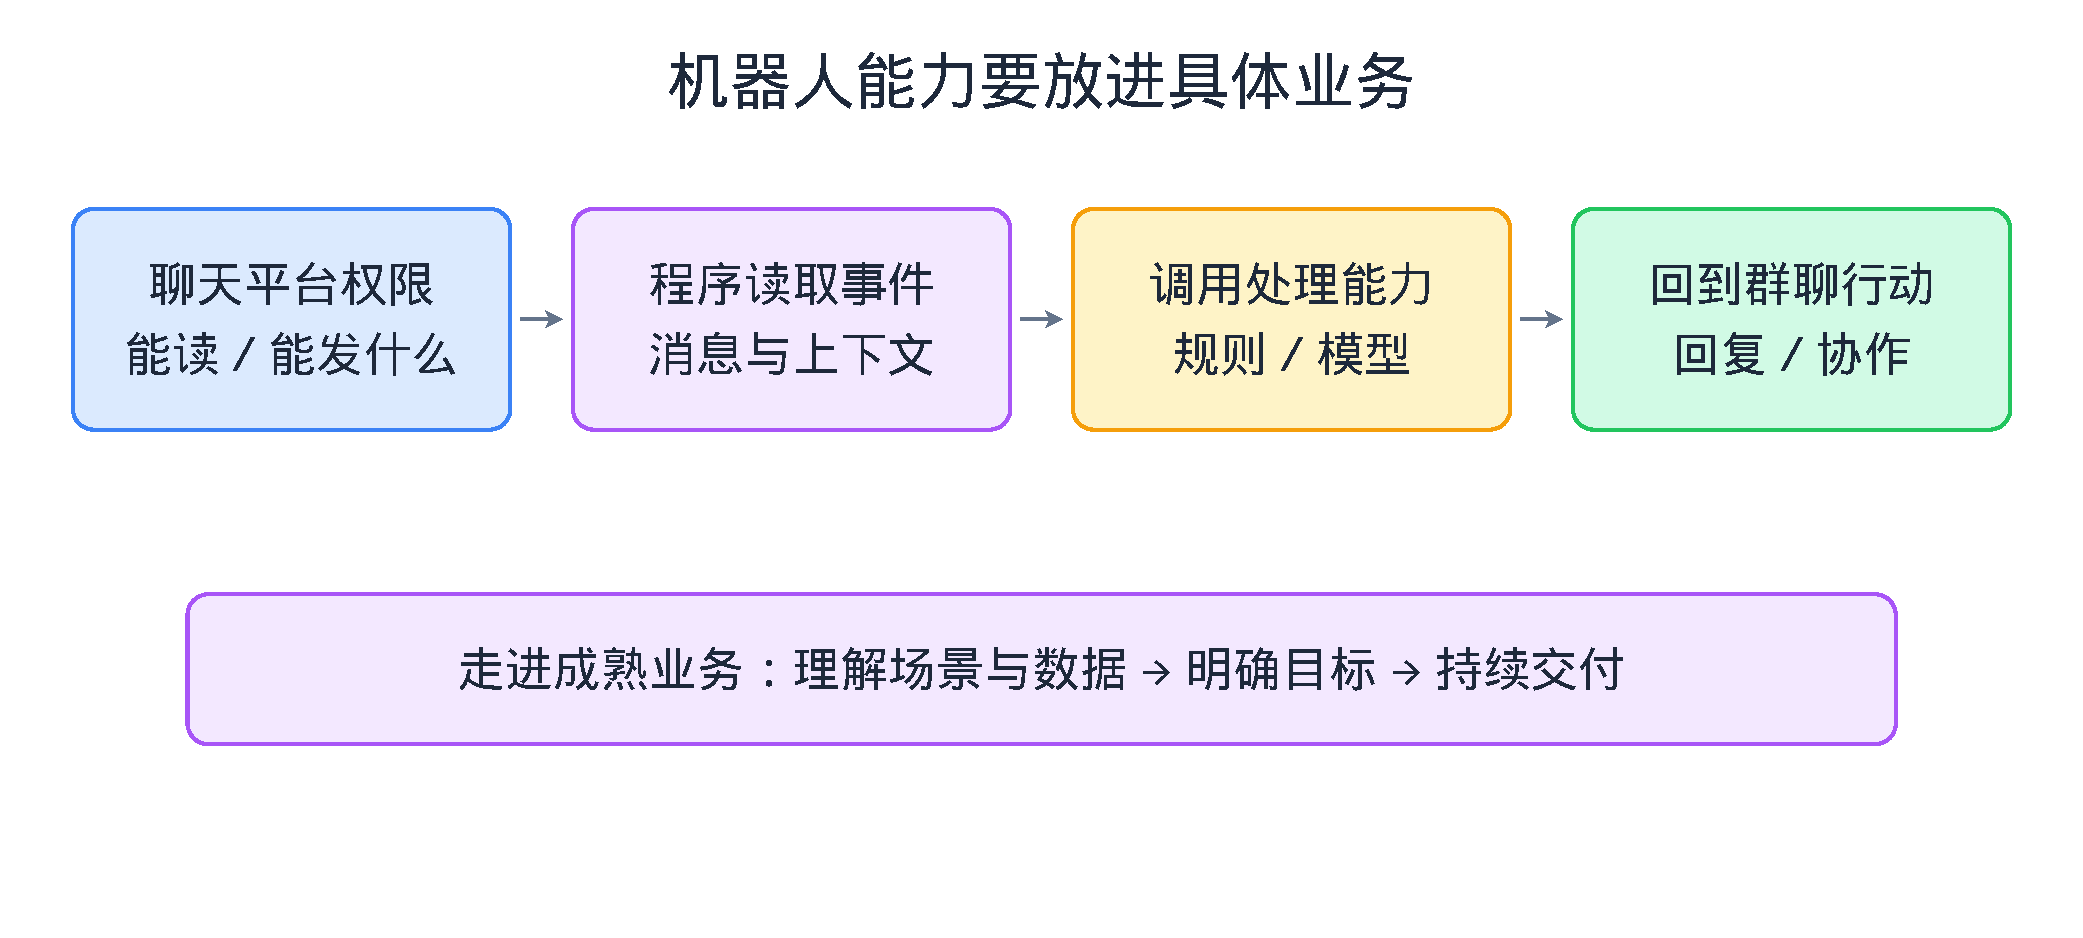
\includegraphics[width=\linewidth,height=.68\textheight,keepaspectratio]{assets/bot-to-business.pdf}
\caption{机器人能力要放进具体业务；依据访谈00:27:09–00:37:18口述整理}
\end{figure}
\begin{knowledgebox}{读图：聊天机器人怎样走进真实业务}
本图分为上下两部分。上方由四个从左到右以实线箭头相连的圆角矩形表示机器人的运行路径：从蓝色框“聊天平台权限：能读／能发什么”，指向紫色框“程序读取事件：消息与上下文”，再指向黄色框“调用处理能力：规则／模型”，最后指向绿色框“回到群聊行动：回复／协作”。下方横跨页面放置一个宽幅紫色框，文字为“走进成熟业务：理解场景与数据 \ensuremath{\rightarrow} 明确目标 \ensuremath{\rightarrow} 持续交付”。
\end{knowledgebox}
可见，群聊Bot能跑通“读取消息—调用模型—回复”的链路只是第一步，要在成熟大厂体系内持续合作，还离不开对业务场景、数据与交付的把握；而在大厂合作中止、融资频频受挫后，创业者又该如何安顿心态并继续行动？
\needspace{6\baselineskip}\subsection{本章小结}
\begin{itemize}
\item \textbf{从具体的平台限制切入尝试}：极群科技起步于陈春宇在2022年前后对聊天软件限制Bot权限的观察，并利用早期Stable Diffusion画风怪异的特点做出了几千名用户参与的群聊互动小游戏。
\item \textbf{认清玩具代码与完整产品的距离}：面对主持人的高看，陈春宇坦承当时并不懂Agent布局、产品化与商业叙事，但这段经历让他重视作为软件使用者和开发者的直觉，保持动手构建（build）的习惯。
\item \textbf{理解成熟业务合作所需的条件}：与百度合作未能持续，并非因为被当成外包，而是早期小团队对大厂成熟业务生态与用户场景理解不足、权限资源有限且缺乏持续交付能力。
\end{itemize}
\needspace{8\baselineskip}\section{承认运气，也保留行动的空间}
在与百度的合作告一段落、重新审视自身产品方向的过程中，陈春宇不仅复盘了业务边界，也谈到了创业者如何看待挫败、运气与日常行动。本章围绕他从奇绩创坛出来后见投资人受挫与初到美国发冷邮件的经历，探讨如何在承认时代与机会随机性的同时，避免把反思变成自我否定，并通过日常的思想实验和具体尝试寻找可落地的切入点。
\needspace{6\baselineskip}\subsection{反思为什么不等于自我否定}
在复盘早期不够成熟的开源运营与大厂合作经历时，主持人月球大叔评价陈春宇具备“向内求”的特质——即遇到阻碍时不抱怨外界环境，而是从自身能力与认知上寻找原因。但陈春宇在访谈（00:37:18–00:38:50）中主动对这一概念做了边界限定：他认为\textbf{过度反思自我并不是一个好习惯}。在他看来，向内反思的核心目的，是把过去的经历与当下的自我整合起来，偶尔从中提炼出一两个能让下一次做得更好的具体改进点，而不是陷入无休止的自我苛责。

如果把“向内求”异化为对过往选择的反复追悔，人就会陷入严重的内耗。陈春宇举例说，如果自己整天纠结“为什么当年没有读人大附中”“为什么没有去北大光华管理学院”，就会永远被困在这些无法改变的假设里。对于外界环境，他主张用\textbf{观察与适应}代替抱怨或苛责：创业者无法控制客观环境的运转规则，但可以盘点自己当下的条件和手牌，选择自己能适应的局部环境去行动。例如，既然没有美国名校背景，那就先设法自己买机票去美国参加活动、与斯坦福大学的学生交朋友，这正是他后来在2024年能够借住在斯坦福宿舍地板床垫上开展项目尝试的现实起点。

\needspace{6\baselineskip}\subsection{努力、机会与成功的归因}
为什么要警惕把所有结果都归结为个人是否努力？陈春宇在00:38:50–00:43:48的对话中，结合合伙人推荐他阅读的迈克尔·桑德尔（Michael Sandel）著作《精英的傲慢》（*The Tyranny of Merit*），谈到了他对“努力与成功”叙事的看法。社会上常有一种声音：既然环境已经提供了机会，一个人没有成功就是因为不够优秀、不够努力。陈春宇明确反对把抓没抓住机会变成一种道德判断或价值判断。他结合自己的求学经历说，如果正常参加高考，自己是考不上清华大学的；当年之所以能保送，是因为他在高中阶段停课学竞赛、赌赢了生物学竞赛。他认为自己后来拿到的一些机会，很大程度上来自尝试之后的\textbf{随机性}，而不能用来证明自己比别人更有道德或更优秀。

为了说明尝试与努力并不一定能直接换来结果，陈春宇分享了两段受挫经历。第一段是在从奇绩创坛出来后，他先后见了150位投资人，结果\textbf{无一例外全部被拒绝}；第二段是他刚到美国、没有任何熟人介绍时，为了联系风险投资机构（VC），发出了200多封\textbf{冷邮件}（Cold Email，指在没有事先认识或引荐的情况下，主动向陌生人发送的联系邮件），最终只有两三个人回复，且\textbf{一个都没有约见成功}（直到后来再次赴美、摸索出针对对方兴趣写冷邮件的技巧后才约上）。他感叹，如果自己是一个斯坦福大学计算机系辍学生（Stanford CS Dropout），当地许多早期基金至少愿意聊聊；而在缺乏这类背景时，现实给出的负面反馈非常强。

面对如此密集的拒绝，如果顺着单一的优绩主义逻辑去想，人很容易产生“我不好”或“社会抛弃了我”的自我否定。陈春宇提到，在硅谷，有些23岁公司估值就达到100亿美元的创业者，容易产生很强的智识与道德优越感，仿佛自己纯粹是因为最积极主动才代表了新时代。但他认为，社会存在分工，不同的人只是在随机性作用下被推向了不同位置；运气好的人如果用“全靠个人努力”的叙事来建立道德优越感，实际上是给那些同样努力却没赶上机会的人强加了一层额外的道德负担。主持人月球大叔对此表示认同，并引用投资界常说的\textbf{盈亏同源}（指在某一阶段带来成功的做法或路径，当环境条件变化后，也可能成为导致亏损或受挫的同一原因）来呼应：从前往后看，人需要认真去做事；但从后往前复盘时，应当承认运气的分量，提醒自己不要迷信过往的做法在任何环境下都会奏效。

\needspace{6\baselineskip}\subsection{用具体尝试检验一个想法}
既然承认了个人能力的局限与外部机会的随机性，这是否意味着一切都归结于运气、无需再反思或行动？陈春宇用了一个比喻来说明随机性与个人尝试的关系：\textbf{“有的时候你要买了彩票才会中奖，但如果你完全不买彩票，你就不可能中奖。”}（00:39:05）在他看来，投入时间和精力去尝试，就像是在买彩票；虽然许多机会都会错失，行动本身也不能保证结果，但只有结合对具体问题的反思去持续尝试，才有可能在随机性作用下抓住一两个小机会，继续留在牌桌上做产品。

在日常做法上，陈春宇在00:43:48–00:48:22介绍了他常做的练习——在“九死甚至九十九死中寻找那一线生机”的\textbf{思想实验}。他在阅读了许多中外企业家与企业的传记后感到，许多公司最终走出来固然有很多偶然因素，但从具体问题出发去推演，往往还能找到尝试的缝隙。例如，在人与人连接的社交领域，微信和Meta看似不可撼动，但他从过往互联网发展案例中形成了一个个人判断：每隔十几年往往会有新的平台出现。当然，他也强调自己并不知道新平台长什么样，如果空想“今天做一个AI原生（AI-native）的微信就一定能打败微信”，那是不可能的；可行的做法是去细想“当前人与人的沟通中还有哪些具体问题没被解决好”，从微小的切入点去大胆假设、小心求证。

\begin{itemize}
\item \textbf{接纳自身局限与差距}：承认自己的平庸、过往的失败以及资源不如人的现实情况，放下精英式的优越感包袱。
\item \textbf{日常高频做思想实验}：哪怕在缺少资金的时候，每天依然围绕目标领域提出假设。任何一个想法都能找出上百个被否定的理由，但可以从中挑出与自己相关、觉得“能做”的具体切口。
\item \textbf{大胆假设，小心求证}：借助现在的AI工具动手做出原型，不去空想直接取代巨头，而是先尝试解决一个具体问题（例如跨语言沟通中的翻译体验），哪怕只在这个领域挖开一个小小的墙角，也是朝目标靠近了一步。
\end{itemize}

这种做法并不要求创业者在第一天就把终局看得一清二楚。主持人在对话中联想到了英伟达（NVIDIA）创始人黄仁勋的传记故事——在华尔街尚不理解、股价经历大幅下跌的时期，黄仁勋依然基于对“计算改变一切”的相信而持续投入\textbf{CUDA}（英伟达推出的通用并行计算架构）。陈春宇接着这一话题表示，很多时候支撑人往下走的是一种\textbf{“模糊的相信”}，如果把所有困难和终局看得太清楚，人反而可能不敢动身了。哪怕当前做的某款小产品最后没有长大，这些在真实尝试中留下的思考与经验，也会像乔布斯所说的“连接人生的点滴”（Connecting the dots）那样，被吸收到后续的经历之中。

\begin{importantbox}{区分“向内整合”与“自我否定”}
陈春宇在回顾150次融资被拒与200多封冷邮件零约见的经历时提到，他的“向内求”主要是把过去的经历与自我整合，并提炼出一两个下次可调整的具体动作（例如：下次发冷邮件时能不能换成对方更感兴趣的话题），同时观察并适应自己当前手牌能触及的环境，而不是把外部条件的限制或未能成事的结果变成对自我价值的否定。
\end{importantbox}
\begin{knowledgebox}{思想实验与最小切口验证}
面对微信、Meta等成熟巨头所在的领域，直接空想做一个替代平台很难落地。陈春宇的做法是通过日常的“思想实验”，在成功概率极低的方向里思考还有哪些具体沟通问题尚未解决，按照“大胆假设、小心求证”的思路，先从翻译等具体切口动手尝试，在实际反馈中一步步推进。
\end{knowledgebox}
\begin{table}[H]\centering\small
\caption{创业归因与行动策略的三种视角对照}
\begin{tabular}{>{\raggedright\arraybackslash}p{\dimexpr(\linewidth-6\tabcolsep)/3\relax}>{\raggedright\arraybackslash}p{\dimexpr(\linewidth-6\tabcolsep)/3\relax}>{\raggedright\arraybackslash}p{\dimexpr(\linewidth-6\tabcolsep)/3\relax}}
\toprule
认知视角 & 解决的问题 & 机制与取舍\\\midrule
优绩主义与精英叙事 & 为世俗成功提供简单的个人努力归因解释 & 将随机机遇完全归功于个人勤奋，易导致成功者产生道德优越感，并给受挫者增加额外心理负担。\\[4pt]
过度内省与宿命论 & 试图通过反复追悔过往选择来解释当前困境 & 纠结于无法改变的出身或学历背景，或者因承认随机性而彻底放弃尝试，导致陷入内耗与行动停滞。\\[4pt]
承认随机性的行动主义 & 在认清资源差距与高失败率的前提下保持创造力 & 接纳平庸与外部条件差距，通过日常思想实验与动手做产品来“买彩票”，结合具体反馈调整做法。\\[4pt]
\bottomrule\end{tabular}\end{table}
从奇绩创坛出来后见150位投资人全部被拒、初到美国发出200多封冷邮件零约见，这类密集的负面反馈很容易让人陷入自我怀疑。陈春宇结合《精英的傲慢》与“买彩票”的比喻，区分了个人可调整的动作与不受控的外部结果。
\begin{figure}[H]\centering
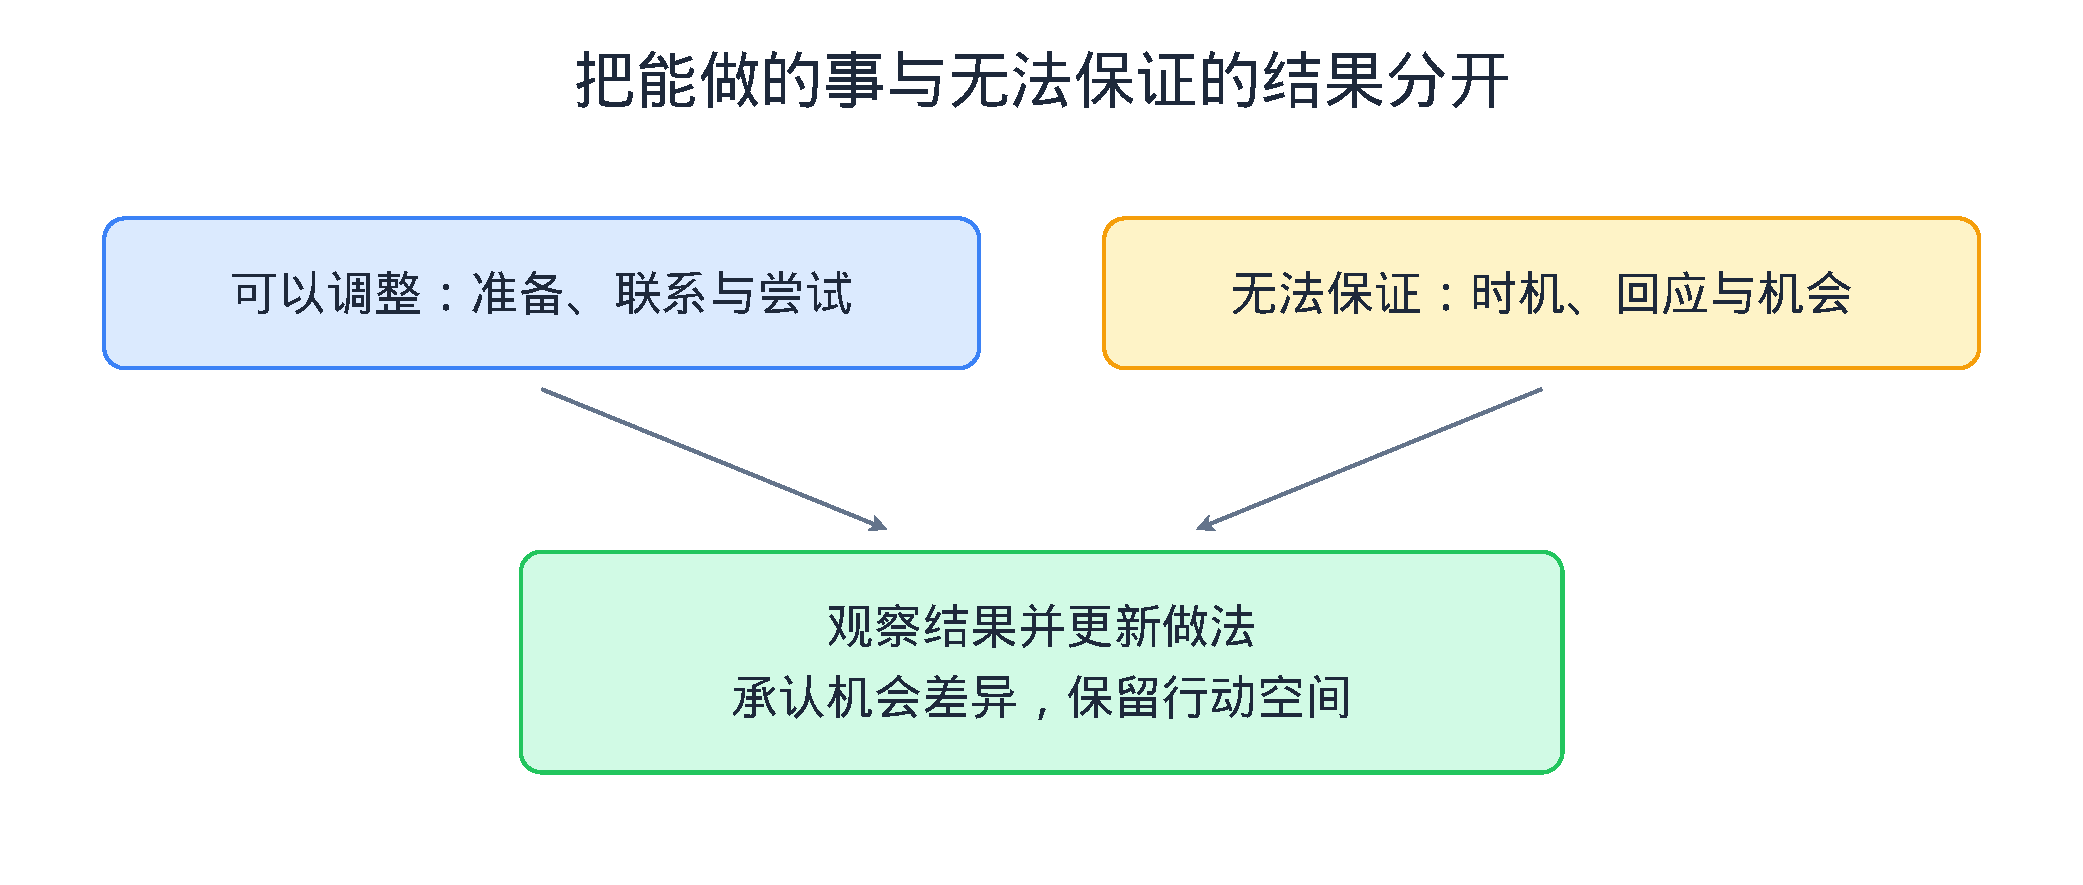
\includegraphics[width=\linewidth,height=.68\textheight,keepaspectratio]{assets/agency-and-feedback.pdf}
\caption{把能做的事与无法保证的结果分开；依据访谈00:37:18–00:48:22口述整理}
\end{figure}
\begin{knowledgebox}{读图：承认运气，也保留行动的空间}
本图呈上二下一的汇聚结构。上方左右并列两个圆角矩形：左侧蓝色框为“可以调整：准备、联系与尝试”，右侧黄色框为“无法保证：时机、回应与机会”。这两个方框各有一条向下倾斜的实线箭头，共同指向下方居中的绿色大框“观察结果并更新做法：承认机会差异，保留行动空间”。
\end{knowledgebox}
把个人能做的准备、尝试与无法保证的时机、回应区分开来，既能避免将坏运气变成自我否定，也能保留修改动作、继续做思想实验与产品求证的空间，这直接引出了第5章的一系列具体产品尝试。
\needspace{6\baselineskip}\subsection{本章小结}
\begin{itemize}
\item \textbf{反思用于自我整合与具体改进}：向内求的目的是把过往经历与自我整合，提炼出下次可改进的具体动作（如调整冷邮件话题），并根据现有条件去适应环境，避免陷入对过往背景的追悔。
\item \textbf{承认随机性，不把结果当作道德判断}：结合《精英的傲慢》与自身150次融资被拒、200多封冷邮件零约见的经历，陈春宇认为机会受随机性影响很大，不应将未能成功等同于不够努力，也需借“盈亏同源”提醒自己不要迷信过往路径。
\item \textbf{在极低概率中做思想实验与具体求证}：承认随机性并非放弃行动，只有动手尝试才相当于“买了彩票”；通过日常思想实验拆解具体沟通问题，靠“模糊的相信”与大胆假设、小心求证持续探索。
\end{itemize}
\needspace{8\baselineskip}\section{从十次尝试中找到具体需求}
承认随机性并保持思想实验的习惯后，接下来的问题是如何把想法变成可验证的产品。本章跟随陈春宇在2023年至2024年间的多次产品尝试，看他如何从无人使用的多智能体框架走向清华早八教室的后排，并在文件整理、菜单翻译与开源Telegram客户端改写的过程中，逐步积累产品设计、前后端工程与消费级应用推广的经验。
\needspace{6\baselineskip}\subsection{走进课堂观察真实使用}
在早期为百度开发聊天机器人的同时，陈春宇团队也在尝试做自己的平台。当时他对开发独立App、处理\textbf{WebSocket}（一种在单个长连接上进行双向通信的网络协议，常用于实时消息收发）长连接或群聊数据库缺乏把握，便从自己能做的网页聊天室做起——最早甚至没怎么用云服务，只跑在单一实例上实现了基础的消息收发，连消息通知都没有。2023年初，团队曾设想构建一个\textbf{Multi-Agent}（多智能体）协作与群体（Swarm）框架，想让Bot与真人平权并在群里模拟小世界，为此编写了\textbf{SDK}（软件开发工具包）和整套文档，还内置了游戏与工具，但结果是没有用户。直到一位清华老师看到他们的网页聊天室，提议将AI与课堂教学结合，团队才得以在清华大学计算机系的一门及几门课上开展尝试。走进真实课堂后，他们发现师生实际需要的是匿名提问、课堂管理，以及结合课本与课件的\textbf{RAG}（检索增强生成，通过检索外部资料库来辅助模型生成回答的技术）问答。由于当时的AI还不够智能，做不到把接口暴露给智能体后由其自主完成全部操作，团队编写了大量中间件脚本，最终将其做成了一款从0到1的独立课堂管理软件。

这款软件在清华上线初期有着数不清的Bug。主持人在对话中打趣说，陈春宇当年离开清华课堂，结果为了这款产品又得在早上八点的第一节课赶回教室。在那个秋季学期，陈春宇每周有好几天在早上七点多起床，赶往清华教室后门观察同学们怎样使用自己的产品。当他从教室后门走进去，看到桌面上每台电脑屏幕都打开着自己的产品界面时，心里很有成就感；但紧接着，他的注意力便会落到异常画面上——哪个界面显示不对、哪个页面报错、谁的账户登不上去。看到报错的瞬间，他形容自己压力陡增、“皮质醇一下就上来了”，立刻从走廊冲到同学面前拍下他们的电脑屏幕、询问账号，并在工作群里急切地与同事排查：“这个账号怎么回事？怎么又登不上去了？为什么这个账号能同时登录两个人？”这种反复在现场排查问题的经历，成了他第一次深入观察用户如何使用产品的起点。他后来觉得，自己在公司里的角色更像是产品经理，当CEO也是为了更好地做产品经理。

在清华找到初步的使用模式后，团队尝试把产品带到斯坦福大学。他们与斯坦福同学合作、住进对方宿舍、一起去上课，在校园里到处贴小广告，往邮件列表（Mail List）里发推广邮件，还爬下了斯坦福3000多门课程的数据做RAG，让用户通过自然语言聊天辅助选课并向学生派发礼品卡，最终获得了2600名用户。但陈春宇形容当时的用户留存“为零”（访谈中未说明具体的留存统计周期，意指大家领完卡试了一下后并没有持续用下来）。尽管当时斯坦福商学院（GSB）一位负责信息系统的主任曾主动发邮件询问能否采购这款软件，释放出早期的正向信号，但陈春宇和团队很快意识到这款专用教学工具再往后做，很可能需要找一批ToB销售去一所所大学挨个推广。他清楚这并不是自己想做的事，尽管这个项目帮他融到了一笔钱并办下了美国工作签证。随着斯坦福的尝试未能持续，团队一度人心涣散，他也在这一时期学会了劝离两位不太匹配的核心成员，重组了团队。

\needspace{6\baselineskip}\subsection{从文件整理到菜单翻译}
在团队士气低落、不知靠什么事情把大家重新聚起来的时刻，陈春宇正好在为准备美国工作签证整理大量繁琐的文件。当时智能体还不像后来那样成熟，他便随手写了一个让AI帮忙整理文件的小脚本，发到小红书、GitHub和推特上，意外火了起来。让他觉得这件事可以继续做成产品的信号，是评论区有人跑来问“这个东西怎么下载、怎么安装”。他起初感到纳闷：“我不是都把GitHub链接发给你了吗，怎么还问怎么下载安装？”但那一瞬间他意识到，即使对于程序员而言GitHub源码也仍需配置环境，而普通用户更需要的是有安装与使用入口、“打开即用”的简单产品。团队借此重新合作了一次，把工具发布到海外新产品发现社区\textbf{Product Hunt}上，不仅获得了产品通讯（Newsletter）的主动报道，还在第一版只做了简单限流、尚未开发付费功能的情况下，邮箱里收到了30多家不同企业的邮件，主动询问如何购买商业授权（Business License）。

看到海外企业对\textbf{SaaS}（软件即服务）的付费询价如此直接，陈春宇当时在心里算了一笔账：他设想如果能把这30多家企业客户转化一半，或许就能达到百万美元\textbf{ARR}（年度经常性收入，将当前订阅收入按年折算的指标，并不保证未来每年稳定不变）的创业小里程碑；甚至如果顺着当时医疗行业潜在客户的需求往下做，也有机会尝试做医疗领域的\textbf{Harvey}（一家法律领域的AI初创公司）。但他当时判断这类通用文件整理工具很可能会被大模型主航道本身的功能演进所覆盖，而且这本来就是一个支线项目（Side Project），他心里真正想做的依然是社交与沟通。当时他的投资人来到客厅找他聊天，陈春宇跟对方讲了这个文件工具的情况，表示新方向还没想好，但可以先把这个事情做好，把投资人投的钱还上。投资人却回答说，根本不在乎这点钱，“你知道我们今年英伟达股票赚了多少钱吗？”并提醒他，当初投他不是为了让他把钱还上，而是因为他当时觉得微信不够好、想做个更好的东西，“你去做吧，我们支持你”。这句话让陈春宇如释重负，放下了“必须靠商业采购和ARR才能假装自己在创业”的心理压力。在那之后，他恶补了大量产品设计与软件工程知识，借助更成熟的大模型，一个人花三周时间写出了一个AI原生即时通讯（IM）应用原型的客户端与后端。那一刻，他觉得自己终于“看见了整只大象”，不再只是摸到尾巴或腿，并靠这个原型Demo筹到了下一笔钱。

在推进IM原型的同时，陈春宇意识到团队在如何把一款2C（面向消费者）应用推向市场，即\textbf{Go-To-Market}（产品触达用户并获取增长的推广过程）上经验为零，便决定挑一个切口简单明确的需求来练手：餐厅菜单翻译。在美国、欧洲和日本，许多餐厅的菜单没有图片，即便认识上面的英语单词，也往往不知道那道菜具体是什么，当时直接用ChatGPT拍照再打字描述也还不够方便。他利用2024年兴起的多模态大模型能力，做出了能够自动搜图、解释菜品，并在拍照后像美团购物车一样把菜品整理出来的菜单翻译应用。在推广上，团队摸索出两条具体经验：一是找TikTok上的小创作者合作，一条未投流、直白介绍产品怎么用的硬广视频爆出了100万播放量，并吸引不少用户付费几美元持续订阅；二是在小红书热门日本餐厅攻略帖子下，让朋友去评论“这家餐厅菜单看不懂，用了这个软件就看懂了”，结果发现这种评论带来的下载量比自己单独发一条内容还要高（这属于他们当时的推广尝试，在实际内容运营中仍需注意平台规则与信息披露边界）。据陈春宇在访谈当时自述，这次菜单翻译练手所积累的短视频获客认知，为后来Intent的Instagram账号做到17万粉丝、Instagram与TikTok双平台合计达到2亿播放量打下了基础。

\needspace{6\baselineskip}\subsection{用使用频率和付费帮助取舍}
通过文件整理学会从0到1做产品经理，又通过菜单翻译摸索了2C应用的推广方式后，陈春宇带着团队回到他最想做的聊天软件上。但从头做好一个即时通讯软件非常困难。这时，AI代码编辑器\textbf{Cursor}已经火了起来，陈春宇在旧金山的一场活动上见到了Cursor的一位联合创始人，了解了他们早期的故事：集成开发环境（IDE）的工程非常复杂（例如VSCode连字符光标都是自己渲染的），而Cursor最早为了快速验证需求，直接\textbf{Fork}（在开源代码库基础上派生出独立分支进行修改）了开源的VSCode。作为Cursor的早期用户，陈春宇记得他们早期的改动带来了不少严重故障——不仅内存占用变得很高，对代码建立索引时有时还会把虚拟机（VM）实例一起带崩溃，导致服务器死机、SSH连接断开。在陈春宇看来，尽管早期版本存在这些严重Bug，但Cursor依然借此验证了用户的核心需求。

受这一思路启发，陈春宇决定在那个阶段先基于开源的\textbf{Telegram}客户端代码，做一个AI版的第三方Telegram客户端。这样做有两个考虑：一方面可以通过研读Telegram虽像“屎山”一样庞杂但功能完备的客户端代码，学习如何构建复杂的客户端工程；另一方面可以直接接入已有的Telegram用户群来做需求验证（当然，基于现有开源客户端改写仍需处理通讯协议、平台规则以及后续向独立应用迁移的问题，同时还要保证基础体验足以让用户走完待验证的任务）。当时，团队把设想到的多种AI助手功能都做了进去：

\begin{itemize}
\item \textbf{群聊事项总结}：自动提炼群组内的关键讨论与待办信息；
\item \textbf{AI智能搜索}：基于语义检索历史聊天记录；
\item \textbf{快捷交互与自动化}：长按任意消息直接向AI提问，以及AI自动备注、自动群管理等。
\end{itemize}

然而，后台数据反映出的使用情况与他们事前的设想不同：上述那些他们原本觉得用户在聊天软件里会常用到的AI助手功能，实际使用频率都很低，用户大约每两三天才会调用一次；在陈春宇看来，这样的频次可以做成插件，但不足以支撑他们想做的独立聊天产品。与此同时，他们意外发现，一个为了防止恶意刷量而顺手加上每月3000条限额、并绑定了付费订阅的\textbf{AI翻译功能}，却有不少用户实实在在地把每月3000条额度用满，并为此付费订阅。当主持人听完这段经历，联想到创业书籍《从0到1》和《创业维艰》里的观点（如“注册不代表留存、留存不代表增长、增长不代表收入、收入不代表能持续活下去”），称赞陈春宇执行了“正确的创业方式”、懂得“及时关掉不对的方向”时，陈春宇对这两点都做出了温和的修正：第一，他认为\textbf{并不存在某种标准的“正确创业方式”}，做决定的那一刻脑子里从来不会去想圈子里流传的方法论，真正指导自己的只有\textbf{如何更好更快地验证用户需求}，以及\textbf{自己真正想做的事情到底是什么}；第二，他认为\textbf{也没有什么绝对“不对的方向”}——比如把此前的PDF文件整理工具继续往医疗领域深耕，或者选择不融资、维持小规模公司，只要知道自己想要什么、知行合一，都是合理的选择。正是基于Telegram测试版跑出的翻译使用与付费反馈，并结合自己做跨语言沟通产品的意愿，他们在开发独立应用Intent的第一版时，砍掉了早期构想的那些AI助手功能，只保留了“翻译”这一项功能。

\begin{knowledgebox}{从GitHub源码链接到普通用户可用的产品入口}
在整理签证文件的案例中，陈春宇最初将写好的小脚本放到GitHub上并附上了链接，但小红书与推特上的读者却纷纷留言询问“怎么下载、怎么安装”。这一反馈让他意识到开发者习惯与普通用户需求之间的差异：即便对于开发者，拉取GitHub代码也往往需要配置运行环境；而对于非技术背景的普通用户或企业人员，他们更需要有明确下载安装入口、打开即可直接使用的产品形态。将脚本进一步封装为易于上手的软件，才促成了后续在Product Hunt上的传播与企业询价。
\end{knowledgebox}
\begin{importantbox}{借助开源客户端代码快速验证功能需求}
当目标产品涉及即时通讯（IM）或代码编辑器（IDE）等复杂客户端工程时，直接从零编写全部基础功能往往耗时漫长。陈春宇从Cursor早期Fork开源VSCode的经历中得到启发（尽管他回忆早期Cursor存在内存占用高、索引偶发导致虚拟机死机等故障，但仍验证了AI编程需求），决定先Fork开源的Telegram客户端代码来挂载各类AI功能。借助现有客户端底座与Telegram用户群，团队在实际使用数据中对比了“每两三天用一次”的总结、搜索等功能与“部分用户每月用满3000条并付费”的翻译功能，从而为独立应用Intent第一版的功能取舍提供了依据。
\end{importantbox}
\begin{table}[H]\centering\small
\caption{极群科技2023—2024年关键试错项目与能力沉淀对照表}
\begin{tabular}{>{\raggedright\arraybackslash}p{\dimexpr(\linewidth-6\tabcolsep)/3\relax}>{\raggedright\arraybackslash}p{\dimexpr(\linewidth-6\tabcolsep)/3\relax}>{\raggedright\arraybackslash}p{\dimexpr(\linewidth-6\tabcolsep)/3\relax}}
\toprule
尝试项目 & 解决的问题与切入场景 & 验证结果与核心取舍\\\midrule
多智能体框架与高校AI助教 & 最初空想智能体平权框架；后落地清华与斯坦福课堂，解决课件RAG问答、匿名提问与选课需求。 & 初期框架零用户；高校助教在清华课堂跑通初步使用，但在斯坦福获2600名注册用户后留存很差（嘉宾形容留存为零，未给统计周期）。因预计后续需靠ToB销售逐校推广且偏离自身志向而停止。\\[4pt]
AI文件自动整理工具 & 针对办签证时繁琐的文件归类痛点，将个人脚本封装为打开即用的桌面工具并发布至Product Hunt。 & 收到30多家企业询问商业授权（嘉宾当时设想若转化一半或可达百万美元ARR，并未实际发生）；判断通用整理易被模型主航道覆盖，在股东支持下回到聊天方向。\\[4pt]
多模态餐厅菜单翻译 & 针对欧美日餐厅无图菜单，利用2024年多模态模型自动搜图、解释菜品并生成美团式购物车。 & TikTok单条硬广视频获100万播放并跑通几美元付费订阅，发现小红书攻略下评论带来的下载量高于单独发帖，积累了2C短视频推广经验。\\[4pt]
AI版第三方Telegram客户端 & Fork开源Telegram代码，集中测试群聊总结、智能搜索、长按问AI、自动备注及AI翻译等功能。 & 总结与搜索等助手功能用户每两三天仅用一次；而防刷量设置的每月3000条限额翻译被不少用户用满并产生付费，遂砍掉助手功能，确立Intent第一版聚焦翻译。\\[4pt]
\bottomrule\end{tabular}\end{table}
在2023年至2024年间，陈春宇团队先后尝试了高校AI课堂软件、文件自动整理工具、餐厅菜单翻译以及AI版第三方Telegram客户端。这些看似跳跃的尝试，各自帮团队检验了哪个层面的问题与证据？
\begin{figure}[H]\centering
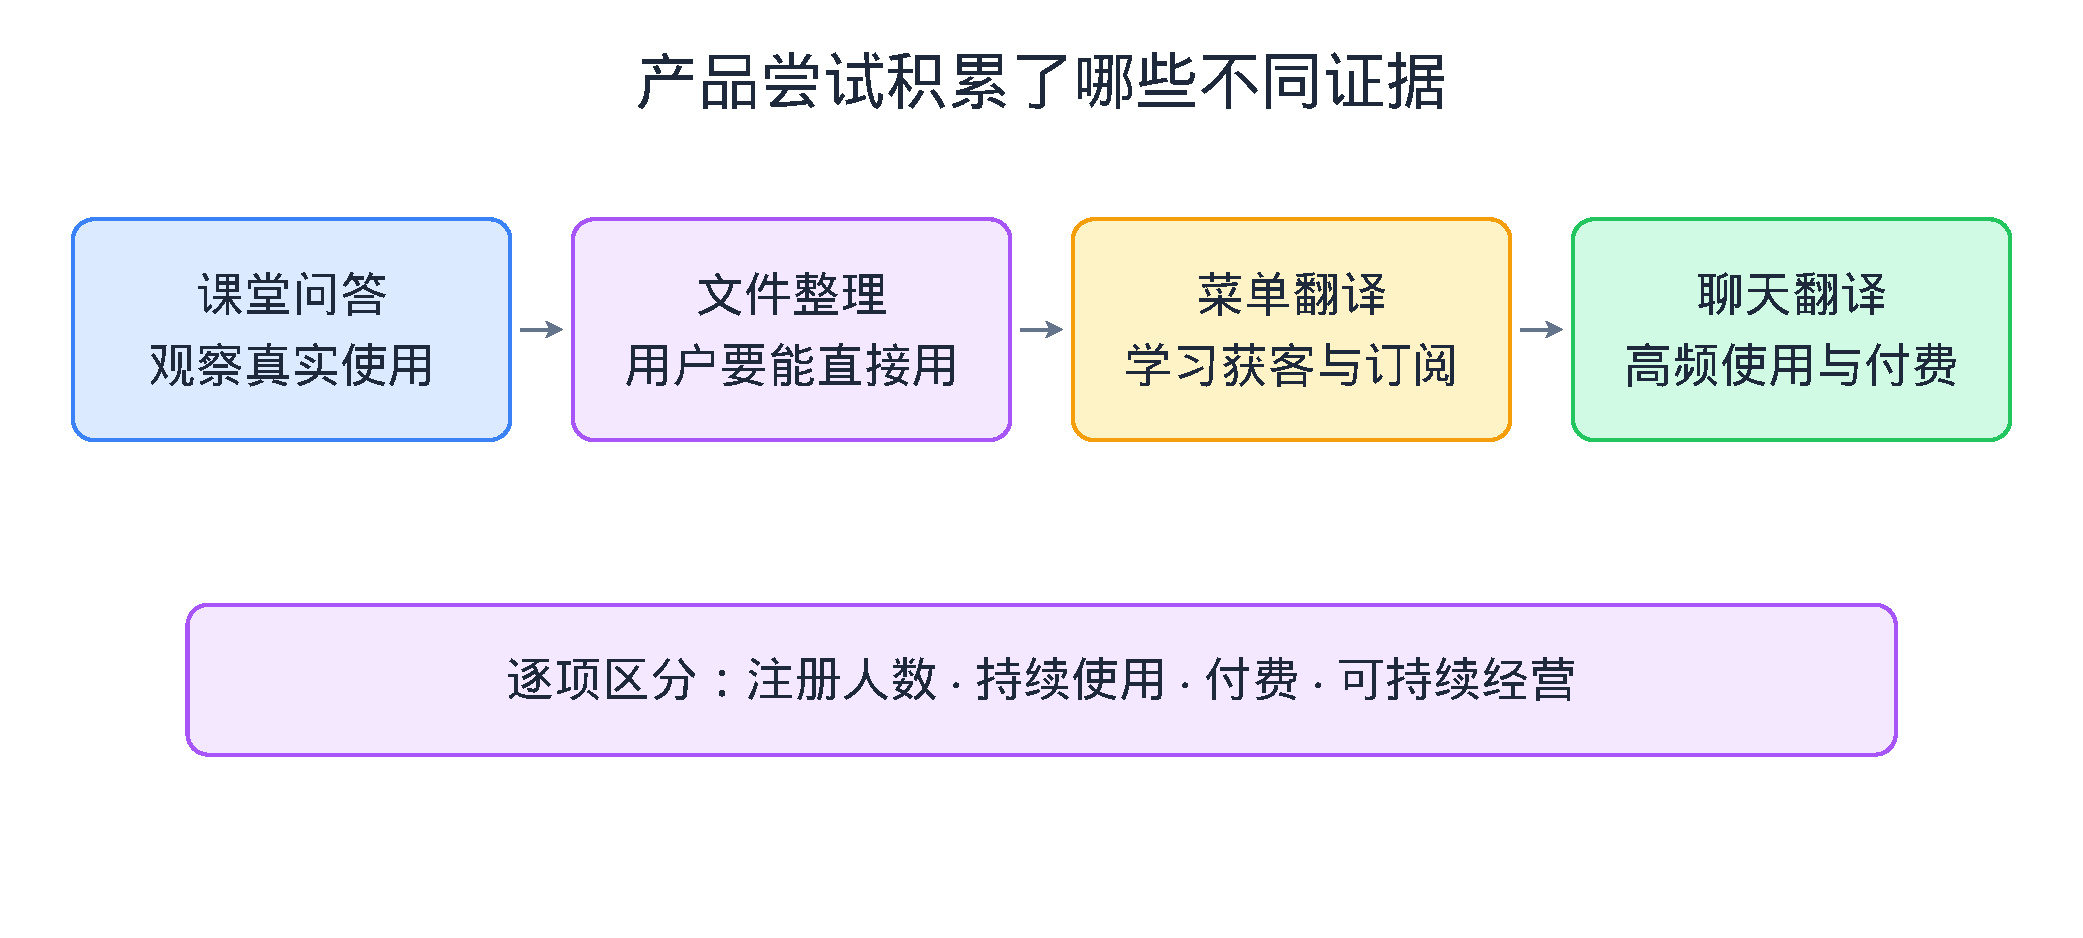
\includegraphics[width=\linewidth,height=.68\textheight,keepaspectratio]{assets/product-evidence.pdf}
\caption{产品尝试积累了哪些不同证据；依据访谈00:48:22–01:07:44口述整理}
\end{figure}
\begin{knowledgebox}{读图：从十次尝试中找到具体需求}
本图分为上下两层。上层从左到右排列四个以箭头相连的圆角矩形，按访谈中的尝试顺序展示四个案例：蓝色框“课堂问答：观察真实使用”指向紫色框“文件整理：用户要能直接用”，再指向黄色框“菜单翻译：学习获客与订阅”，最后指向绿色框“聊天翻译：高频使用与付费”。下层放置一个宽幅紫色框，写明“逐项区分：注册人数 · 持续使用 · 付费 · 可持续经营”。
\end{knowledgebox}
通过逐项区分注册人数、持续使用、付费意愿与可持续经营，团队在Telegram测试版中识别出高频且有人付费的翻译需求，并由此进入第6章对独立跨语言沟通应用Intent的打磨。
\needspace{6\baselineskip}\subsection{本章小结}
\begin{itemize}
\item \textbf{走进真实使用现场观察问题}：告别早期零用户的多智能体SDK设想，通过每周数次早起去清华早八教室后门看学生屏幕、排查报错，以及去斯坦福测试选课与留存，积累了从0到1观察真实用户交互的经验。
\item \textbf{在具体小项目中补齐工程与推广能力}：从文件整理脚本被追问“如何安装”意识到用户需要直接可用的产品，靠三周独立写出IM原型前后端摸清聊天软件的整体结构，并通过菜单翻译在TikTok与小红书试出了短视频获客与小额订阅路径。
\item \textbf{结合使用数据与个人志向做功能取舍}：借鉴Cursor早期Fork VSCode验证需求的思路，基于开源Telegram客户端测试多项AI功能；根据实际使用数据（两三天一次对比不少用户月满3000条并付费）砍掉助手功能，同时明确创业并无唯一标准方式，关键在于更快验证需求并想清楚自己真正想做的事。
\end{itemize}
\needspace{8\baselineskip}\section{翻译之外，怎样帮助人们沟通}
通过前期的多次产品尝试与开源客户端验证，陈春宇团队砍掉了使用频次较低的AI助手功能，将Intent的第一版聚焦在跨语言翻译上。当主流通讯软件同样具备翻译功能时，初创团队如何做出让部分用户愿意持续使用的产品？本章从日常聊天的上下文（Context）积累、语音与文本翻译的技术链路，以及走进西语裔社区和ESL课堂的用户观察三个方面，梳理他们如何围绕跨语言沟通打磨细节，并思考字面翻译之外的意图理解。
\needspace{6\baselineskip}\subsection{把翻译放进日常沟通}
在验证了翻译功能的付费意愿后，为什么陈春宇依然选择投入2C（面向消费者）聊天软件，而不是去做企业级工具？在他看来，自己想解决的是“人与人之间的连接”，而聊天软件正是承载真实关系、沉淀大量\textbf{Context（上下文背景信息）}的高频刚需场景。他在访谈中举了一组数字来说明聊天场景的交互密度：在WhatsApp上，每个用户平均每天发送60多条消息；而在Intent上，他们的核心用户每天发送的消息量已达到57条（需要注意，Intent的“核心用户”与WhatsApp的“全体平均用户”统计口径不同，不能直接等同比较两者的整体黏性）。相比之下，普通用户很难在Twitter（现X）或Instagram Story上每天发60条内容；即便是ChatGPT，在他们当时看到的数据里人均单日交互也只有十来条，因为人与AI对话缺少人际社交的触发机制（Social Trigger），聊着聊着容易没话题，即便一些AI伴侣或互动应用尝试通过引入外部事件来激发对话，在当时的效果也还不算出色。

面对投资圈里“每隔五六年或十年就会出现新一代聊天产品”的说法，陈春宇明确表示，自己并没有笃定地相信AI时代一定会出现新的社交巨头，也不是为了追求未来被大厂以几百亿美元收购的商业价值。他把“聊天产品会换代”当作一个既无法证明也无法证伪的个人信念，把日常精力放在思考“聊天里还有哪些需求没被解决好”上。当不少开发者选择做更容易拿到GitHub星标和融资的\textbf{Agent Harness（智能体运行与编排框架）}，或者因为忌惮Meta与微信的体量而避开聊天赛道时，他的感受是“别人是在算账，而我在看问题”。比如，他觉得现在的社交世界太吵闹，人们需要一个更好的沟通“转换器”；为此，他去读华盛顿大学心理学家约翰·戈特曼（John Gottman）关于亲密关系与婚姻冲突的理论，尝试在团队内部探讨“社交弱互动”等改善连接方式的思路。

为了理解不同年龄段用户的沟通习惯，Intent团队在人员构成上保持了较大的年龄跨度：既有不到20岁的年轻成员，也有在实现稳定消息收发和客户端优化上经验丰富的工程前辈，陈春宇则在中间结合自己对05后、10后的理解与对前沿多模态模型能力的跟踪来衔接产品方向。通过邀请部分用户分享聊天记录，他在这些样本中观察到一些现象：例如一些10后青少年会把豆包或ChatGPT当成生活百科全书，随时询问“这个菜能不能吃”“这只鸟叫什么”，这与职场人用AI写邮件、处理账单的习惯很不一样；同时，在他接触到的样本里，不少老人、小孩以及非技术背景用户在收到AI回复后，常会回复一句“谢谢”。在上下文缓存（Caching）做得不够好时，这种礼貌寒暄会带来可观的额外\textbf{Token（大模型处理文本的基本计算与计费单元）}消耗；陈春宇对此的感触是，部分用户确实把AI当成了可对话的实体，相比之下，一位程序员在用Cursor改完代码后通常不会专门再去跟编辑器说声谢谢。

\needspace{6\baselineskip}\subsection{语音链路与真实用户评价}
既然WhatsApp和Instagram等主流应用本身也有翻译功能，用户为什么还会用Intent？陈春宇表示，团队完全没有按照“怎么和巨头打仗”的逻辑去想问题，而是因为一些用户觉得现有软件里的翻译不够顺手。他坦言自己英语不好，更不会其他小语种，但有巴西、韩国等世界各地的朋友，在日常联系中能体会到怎样设计更顺手。比如，Intent让双方各自使用母语交流（对方说韩语、自己说中文，界面上各自看到译为自己语言的内容），并做成了自动翻译以及自动语音转文字再翻译的流程，省去了反复手动操作的麻烦。这种围绕具体痛点的细节设计，让一部分跨国伴侣、家人和挚友把重要关系放在了他们的软件上。

当跨语言聊天从文字延伸到语音时，完整的技术链路通常串联起三个环节：\textbf{语音识别（ASR，Automatic Speech Recognition，输入说话人的源语言音频，输出源语言文本）}、\textbf{文本翻译（输入源语言文本，结合上下文输出目标语言文本）}，以及\textbf{语音合成（TTS，Text-to-Speech，输入目标语言文本，输出合成的目标语言音频）}。主持人在访谈中提出设想：如果韩国朋友说韩语，自己听到的不仅是翻译后的语言，还能通过\textbf{音色克隆（Voice Cloning，在语音合成中模仿说话人的声线特征）}保持对方原本的音色与情感，体验会非常好。陈春宇回应说，他们目前已经接入了带声音克隆的TTS，在中英互译上的音色克隆效果已经做得还不错，但他对整体效果尤其小语种之间的表现还不太满意。他推测这主要是训练数据源的问题——例如在将西班牙语翻译并合成为中文语音时，出来的声音有时听起来很像“台湾翻译腔”，他猜测这可能是因为模型使用了YouTube上的繁体中文配音视频作为数据源。

陈春宇表示，在节目当时提到的400万用户规模下（访谈中未说明该数字是累计下载、注册还是其他统计口径），团队还不足以投入巨资去训练自己的底层语音基座模型，但他设想如果未来商业化验证跑通、积累了足够的资金和资源，也可以尝试训练自己的TTS模型。更重要的是，真实聊天场景中的用户反馈已经帮他们发现了通用评测之外的问题。陈春宇分享了一个内部评测结果：在他们基于真实用户打分构建的内部\textbf{Benchmark（评测基准）}上，知名语音AI公司ElevenLabs的新版V3模型，在Intent的真实用户评分中表现反而不如旧版的V2模型。这一在具体跨语言聊天场景下由用户打分反映出的差异，是模型厂商在通用测试里未必能直接注意到的。

\needspace{6\baselineskip}\subsection{接近用户的生活与表达}
为了真正理解跨语言用户在怎样的生活环境中交流，陈春宇在赴美开拓市场的过程中，没有把观察局限在硅谷科技圈的熟人圈子里。他的用户观察方式受到清华本科大二一门名为《舌尖上的社会学》的课程影响，特别是其中接触到的法国学者布鲁诺·拉图尔（Bruno Latour）在《实验室生活》中谈到的\textbf{“陌生化”}视角——陈春宇将其形容为跳出自己高三就习以为常的实验室认知，就像假设自己是一只拿着“会发光的砖头（手机）”的猩猩那样，先放下“我早就知道手机怎么开关机、按钮干什么用”的预设，去观察人们在真实生活里如何使用工具。因为自己是清华生物专业背景，刚来美国时不像计算机名校毕业生那样有许多在Meta、Google工作的师兄师姐，他在美国甚至主动在建材超市Home Depot门口，用夹杂着西班牙语单词的英语跟讲西语的墨西哥裔人士搭话。在聊天中他注意到，对方手里用的并不是iPhone，而是三星Galaxy A56；他提到，如果去亚马逊上买一台那样的三星A56，会发现那台机器的默认语言设置就是西班牙语。

通过这种日常接触，他与一位曾有过酗酒经历、后来戒酒并考取了心理咨询师执照的园丁成了互送礼物的好朋友。在园丁的带领下，陈春宇走进了当地的Hispanic（西语裔）社区，在产品正式上线前邀请园丁的朋友以及十几岁的孩子帮忙测试TTS语音功能。在走进用户家里的过程中，他感到理解用户不能只靠坐下来问“你怎么跟家人联系”，而是去留心他们居住的街区、收拾得干净整洁的房间、家里有几口人以及交谈中强调或回避的话题，在自然相处中感受对方的生活状态。此外，在一位曾在斯坦福大学心理系做过研究的团队成员协助下，英语本就是第二语言的陈春宇还报名去当地社区学院上\textbf{ESL（English as a Second Language，以英语为第二语言）}课程。在课上，他遇到了许多努力追求更好生活的移民，比如希望学会直接用英语跟雇主沟通、避免再被中介剥削的住家保姆，在与他们一起上课的过程中体会跨语言沟通的实际困难。

在经历了这些面对面的交流后，陈春宇觉得现有的翻译工具（包括目前的Intent）都还不够好用。他在访谈中引用了“语言即思维”的说法来表达自己的感受，而主持人在交流中也谈到不同语言在语序（如主谓宾SVO与主宾谓SOV）和表达习惯上的差异——有的表达直白，有的则包含言外之意。陈春宇进一步提到，之所以把公司取名为Intent（意图），是因为他发现即便讲同一种语言、甚至彼此已经非常熟悉的人，在说同一句话时也常常因为不理解对方的真实意图而产生冲突。针对主持人提出“恋爱与人际交流的美感有时正来自若有似无的含蓄，过于直白地拆解意图是否会成为双刃剑”的疑问，陈春宇认为，工具如何被使用最终取决于用户自己的选择——就像Instagram的Story或微信朋友圈允许人们选择性地浏览朋友动态，而不必把每一天的所有细节都塞进聊天框一样，未来的沟通工具在用户需要准确传达意思时可以提供帮助，在用户希望保留模糊与分寸感时也可以把选择权留给个人。

\begin{knowledgebox}{跨语言语音聊天的三段式链路（ASR—翻译—TTS）}
在聊天软件中实现“一方说母语语音、另一方听目标语言语音”，概念上需串联三个环节：
\begin{enumerate}
\item \textbf{语音识别（ASR，Automatic Speech Recognition）}：输入说话人的源语言音频，输出对应的源语言文本。
\item \textbf{文本翻译}：输入源语言文本，结合对话上下文（Context）与语境，输出目标语言文本。
\item \textbf{语音合成（TTS，Text-to-Speech）}：输入目标语言文本，输出目标语言音频；若配合音色克隆技术，则尝试模仿说话人原有的声线特征。

\end{enumerate}
在实际聊天中，用户不仅关心译意是否准确，还会直接感受合成声音是否自然（如陈春宇猜测某小语种转中文带“台湾翻译腔”可能与训练数据源有关），以及整条链路走完的总等待时长是否影响对话节奏。因此，依靠真实用户在具体聊天场景中的打分来评估模型（如团队内部测出ElevenLabs V3得分低于V2），能补充通用评测难以覆盖的体验细节。
\end{knowledgebox}
\begin{importantbox}{基于“陌生化”视角的田野用户研究}
受人类学民族志与拉图尔《实验室生活》启发，陈春宇在了解跨语言用户时采取了走出科技圈的做法：
\begin{itemize}
\item \textbf{悬置预设（陌生化）}：不把硅谷常见的iPhone或纯英文环境当作默认前提，在日常接触中留意对方实际使用的手机型号与语言设置。
\item \textbf{进入真实生活与学习场景}：不局限于结构化问卷，而是通过日常搭话、与社区园丁交朋友、亲自去社区学院上ESL（以英语为第二语言）课程等方式，在自然相处中理解移民群体学语言、找工作与联系家人的需求。
\item \textbf{邀请社区用户参与早期测试}：在产品上线前，请社区里的朋友及其家人实际试用TTS语音等功能，收集真实生活场景下的反馈。
\end{itemize}
\end{importantbox}
\begin{table}[H]\centering\small
\caption{跨语言聊天与沟通辅助中的四类任务及产品取舍}
\begin{tabular}{>{\raggedright\arraybackslash}p{\dimexpr(\linewidth-6\tabcolsep)/3\relax}>{\raggedright\arraybackslash}p{\dimexpr(\linewidth-6\tabcolsep)/3\relax}>{\raggedright\arraybackslash}p{\dimexpr(\linewidth-6\tabcolsep)/3\relax}}
\toprule
沟通任务与功能层次 & 主要解决的沟通问题 & 运行机制与产品取舍\\\midrule
双向自动文本翻译 & 减少跨语言日常文字聊天中手动复制或逐条点击翻译的操作步骤 & 双方各自输入母语，界面直接向对方呈现译文；服务于跨国伴侣、亲友等高频联系，是Intent第一版保留的核心功能。\\[4pt]
语音转译与音色合成（ASR \ensuremath{\rightarrow} 翻译 \ensuremath{\rightarrow} TTS） & 支持用户在不便打字或习惯发语音时直接用母语说话并以对方语言呈现 & 串联语音识别、文本翻译与语音合成（含音色克隆尝试）；中英效果较可用，但小语种仍受数据源口音与整体等待时长制约，需靠真实用户打分持续筛选模型。\\[4pt]
高频对话中的上下文（Context）与代际理解 & 适应不同年龄与技术背景用户在日常聊天及AI交互中的习惯差异 & 依托真人聊天积累的上下文；针对样本中部分用户常对AI说“谢谢”等习惯，需做好上下文缓存以控制额外Token消耗。\\[4pt]
字面翻译之外的意图（Intent）传达与表达选择 & 缓解跨文化或同语种熟人交流中的言外之意误解与社交吵闹感 & 参考亲密关系理论探索“社交弱互动”与沟通转换器；在帮助说明真实意图的同时，把直白沟通或保留含蓄留白的选择权交给用户。\\[4pt]
\bottomrule\end{tabular}\end{table}
当跨语言沟通从文字延伸到语音时，用户不仅关心字面意思对不对，还会直接感受到声音是否自然、等待是否过长。Intent在接入语音识别、翻译与语音合成模型时，如何借助真实用户反馈来评估和改进体验？
\begin{figure}[H]\centering
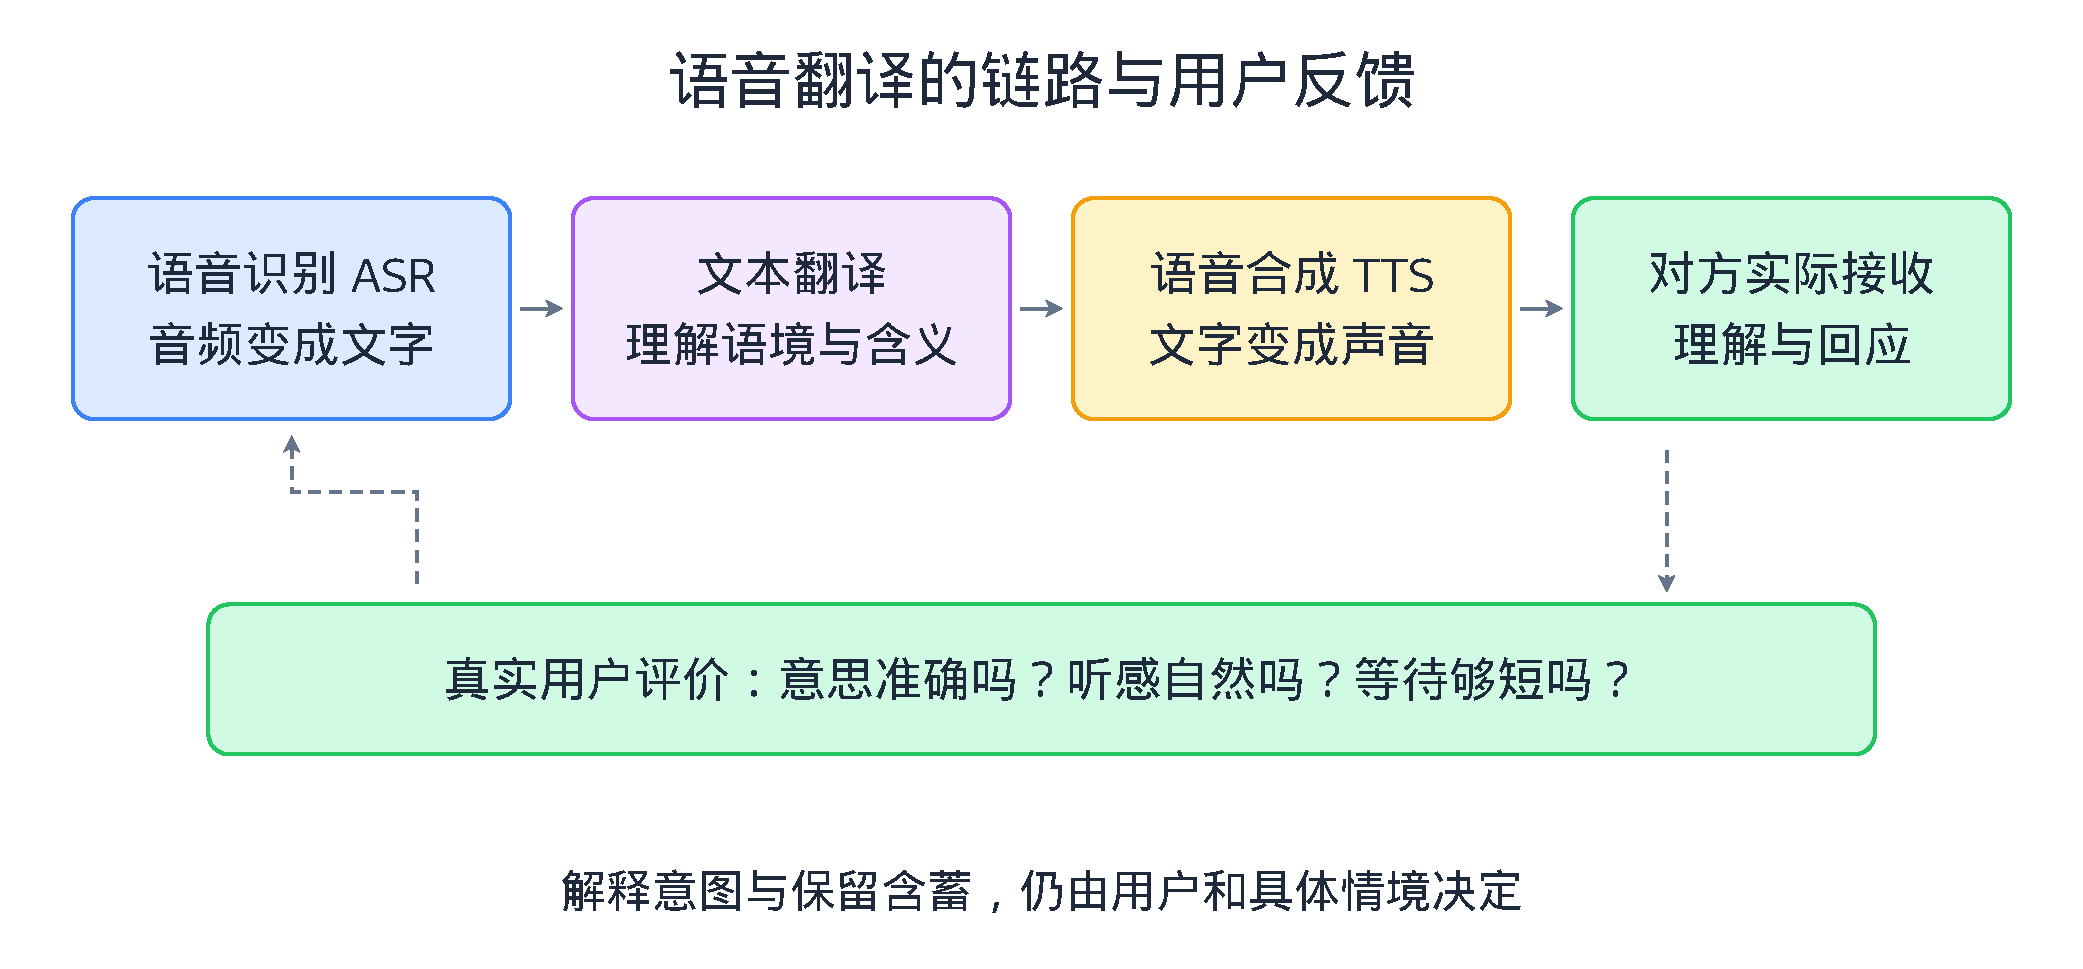
\includegraphics[width=\linewidth,height=.68\textheight,keepaspectratio]{assets/communication-loop.pdf}
\caption{语音翻译的链路与用户反馈；依据访谈01:16:00–01:38:04口述整理}
\end{figure}
\begin{knowledgebox}{读图：翻译之外，怎样帮助人们沟通}
本图构成一个带反馈的闭环。上方从左到右四个由实线箭头相连的方框展示语音转译链路：蓝色框“语音识别 ASR：音频变成文字”\ensuremath{\rightarrow}紫色框“文本翻译：理解语境与含义”\ensuremath{\rightarrow}黄色框“语音合成 TTS：文字变成声音”\ensuremath{\rightarrow}绿色框“对方实际接收：理解与回应”。下方有一个宽幅绿色框“真实用户评价：意思准确吗？听感自然吗？等待够短吗？”；右侧一条虚线箭头从“对方实际接收”向下指向该评价框，左侧另一条虚线折线箭头则从评价框向上指回“语音识别 ASR”框。最底部有一行文字：“解释意图与保留含蓄，仍由用户和具体情境决定”。
\end{knowledgebox}
正是通过“对方实际接收\ensuremath{\rightarrow}真实用户评价\ensuremath{\rightarrow}反向定位ASR、翻译与TTS问题”的反馈回路，团队发现了通用模型在实际聊天中的评分差异；而支撑团队在多次试错中走到这一步的心理与团队基础，将在第7章展开。
\needspace{6\baselineskip}\subsection{本章小结}
\begin{itemize}
\item \textbf{看重真人聊天的高频连接与上下文积累}：选择投入2C聊天产品，是因为看重人与人日常连接对普通人的意义以及聊天场景沉淀的丰富上下文（Context），而非笃信社交巨头换代或追求收购估值。
\item \textbf{通过真实用户打分打磨语音与翻译链路}：串联语音识别（ASR）、文本翻译与语音合成（TTS）降低跨语言交流的操作摩擦；依靠真实场景的用户打分评估模型表现（如发现ElevenLabs V3在内部评分中不及V2），并留意小语种合成中的口音问题。
\item \textbf{走近真实社区用户并尊重表达边界}：借鉴人类学“陌生化”视角，通过与西语裔社区园丁交友、邀请家庭测试及同上社区学院ESL课程来理解用户处境；在探索意图（Intent）传达时，把直白解释或保留含蓄的选择权留给用户。
\end{itemize}
\needspace{8\baselineskip}\section{相信自己，也学会与他人一起走}
前两章梳理了陈春宇在多次产品尝试中的验证过程与走进社区的用户观察。在多次调整方向、经历成员变动与缺乏正向反馈的时期，创业者依靠什么维持状态？本章回到访谈后段（01:07:44–01:16:00，01:41:21–01:53:44），看他如何剖析自己从单一优等生标签走向自我接纳的过程，如何通过亲自学习补齐产品与工程短板来减少半途妥协，以及如何在硅谷冷启动环境中依靠相识于微末的合伙人与稳定的自我关怀继续前行。
\needspace{6\baselineskip}\subsection{从优等生身份走向自我接纳}
面对多次方向调整、部分早期成员离开与持续缺乏正反馈的经历，主持人提问是什么支撑他一次次继续尝试而不选择停下来休息。陈春宇在访谈（01:08:20–01:15:24）中用日常语境下的“自恋”一词来形容自己的心力来源，并解释说那是指一种来自内心深处的自我认同与自我价值实现愿望（并非临床心理学上的诊断概念）。他对比了自己在不同阶段的状态：在刚刚通过竞赛保送清华或本科早期发表论文时，他的自我认同是单一且单薄的，主要来自“比你们都早进实验室、在本科就发了更好的论文”；而在与社会有了更多互动、经历过诸多打击后，他意识到自己能够承担责任、体会他人情绪、看见不同人群的生活视角，并从喜欢的同事身上学到很多东西，把这些不同部分整合在一起，成了更完整的自己。

这种对自我不同侧面的整合，也影响了他对做事方向与团队协作的看法。陈春宇谈道，如果只是因为风口来了让公司估值翻倍，夜深人静向内审视时，创始人未必觉得自己作为一个人在变好；而在一次次熬过否定与选择的过程中，他承认人当然也会有脆弱，但自己从中感受到了一种踏实的力量感。他觉得，既然自己同时在学数学、大模型原理，也在看人文社科书籍并做用户研究，那与其只把早期的PDF文件整理工具往百万美元ARR的设想上推进，不如去尝试自己真正想做、对综合能力要求也很高的2C聊天产品。在团队内部，他以前曾尝试亲自去调停同事之间的矛盾，后来发现那会让自己陷入过度消耗，便学会了调整边界。遇到解决失败的问题时，他笑称自己也会找借口缓冲一句“没关系，反正大部分人都没做成”，同时在做成的小点上给自己正反馈。

\needspace{6\baselineskip}\subsection{用学习与验证建立信心}
在总结七次乃至近十次产品尝试的最大经验时（01:41:21–01:47:27），陈春宇给出的回答是\textbf{更相信自己}。他反思，早期推进一些项目时之所以只验证了一半，往往是因为信念感（Conviction）不够，或是与团队出现意见分歧时轻易做了妥协方案。最初他先后对自己的产品能力和技术能力不够自信；但随着团队成员教他、借助AI工具学习，以及自己去修读计算机系统等课程，他发现产品、软件工程、架构思维、云服务使用乃至心理学和融资知识都是可以习得的，现在自己已经能够从零到一写出支撑一定用户规模的前后端代码。

陈春宇特别说明，作为CEO“少做妥协”绝不是在公司里搞一言堂、强迫所有人必须按某个方向做否则就开除；真正的做法是当大家还不知道这件事怎么能做成时，创始人自己去探索，通过亲自学习或招募合适的人把缺失的环节（Gap）补上，用跑通的事实、信念感和感染力说服团队一起往前走。主持人听后也分享了自己的经历：他在Claude Code出现前一年也曾做过一款冲上GitHub榜单的开源命令行界面（\textbf{CLI}，Command-Line Interface，通过文本指令与程序交互的工具），当时他就相信CLI代表着生产力方向，但因为不够自信，没有鼓起勇气去融资创业和说服身边人一起投入。两人还交流了如何看待成败：虽然信念和坚持并不能保证创业成功，现金流与用户反馈依然是生存的现实基础，但陈春宇认为，在日常心态上可以把未达预期定义为“下次可以做得更好”，不必因为看到新闻里别人用户量更大、融到更多钱就觉得自己彻底失败，而是关注自己在想做的方向上有没有比昨天更进一步。

\needspace{6\baselineskip}\subsection{合伙人的支持与生活排序}
个人的探索也离不开投资人与合伙人的支持。在01:41:21–01:42:54与01:49:43–01:52:00的对话中，陈春宇坦言公司能活到现在确实依靠投资人的持续支持。他能体会投资人在看到团队做出的东西与年初所说不同时的怀疑与担心——有的投资人曾直接督促他把迭代和验证的速度提得再快一点，也有投资人一边心里慌张，一边又怕给他太大压力而在口头上鼓励“春宇好好干，我们相信你”；他把这种关系看作在艰难创业路上的互相陪伴、并肩前行。而在团队内部，虽然早期有意见不合的成员离开，但他核心的合伙人从未换过，都是很早就认识并一路一起打拼下来的。有一年年底情况非常困难，合伙人甚至觉得公司快要撑不下去了，做好了“陪春宇走完最后一程”的准备，直到他在年底又融到一笔钱才得以继续做下去。

这种相识于微末的信任在硅谷的冷启动环境中显得格外珍贵。谈到国内看重的清华光环，主持人与陈春宇聊到了外来创业者在硅谷的实际感受：如果没有进入Y Combinator（YC）、a16z、红杉（Sequoia）或Benchmark等当地核心创投圈子，依然得一步一步从头走起。陈春宇讲了一个身边的例子：他们曾招过一位白人技术同事，对方虽然知道清华不错，但原本一直以为清华只是和加州大学戴维斯分校（UC Davis）差不多的学校；他个人还觉得，在大模型热潮之前，如果去硅谷找传统的软件工程工作，清华背景在当地的认知度有时甚至不一定比得上印度理工学院（IIT）。谈完这些经历，陈春宇在访谈最后（01:52:00–01:53:44）回答了“人生最重要的是什么”：对他来说，首先是学会爱自己。他觉得，当自己学会爱自己、并在一个稳定被爱的环境中获得支持时，首先能为身边最亲近的家人、同事和未来的伴侣创造好的情绪与物质条件；再往外一圈，当同事和股东看到事情一步步变好、获得体面收入与回报时，大家也会更有动力通过团队协作做出对世界有积极影响的事情，把这份力量感一圈一圈地向外传递。

\begin{knowledgebox}{命令行界面（CLI）与创始人亲自补齐工程短板}
\textbf{命令行界面（CLI，Command-Line Interface）}指用户通过输入文本指令与计算机程序交互的界面，区别于主要依赖图形按钮或单纯对话网页的交互方式。当CLI工具在设计上接入本地开发工具链并获得相应授权时，开发者可以直接在终端环境中调用脚本与处理工程任务，这也是主持人在访谈中提到的生产力工具方向。

在早期团队协作中，陈春宇提到的经验是\textbf{亲自补齐工程与产品短板}：通过向同事请教、借助AI辅助学习以及修读计算机系统等课程，让自己具备从零到一编写前后端原型与理解云架构的能力。这样在团队对某个想法的技术可行性存疑时，创始人可以通过亲自动手把缺失环节（Gap）跑通，用实际结果与团队沟通。
\end{knowledgebox}
\begin{importantbox}{减少决策妥协与“一言堂”的边界}
在复盘多次产品尝试时，陈春宇提出“更相信自己、少做妥协”，并明确解释了这与专断命令的区别：
\begin{itemize}
\item \textbf{减少半途而废的折中}：早期因对自己的产品或技术能力不够自信，遇到团队意见分歧时容易采取折中方案，导致想法只验证了一半。
\item \textbf{不搞行政“一言堂”}：少做妥协绝不是强令所有人服从、谁不服从就开除谁，而是避免在不理解技术与产品细节的情况下强行下令。
\item \textbf{亲自填补空白（Gap）}：当大家还不清楚一件事怎么能做成时，创始人通过自己去学、去招合适的人把卡住的环节跑通，再用验证清楚的结果与信念感说服团队一起推进。
\end{itemize}
\end{importantbox}
\begin{table}[H]\centering\small
\caption{创业支撑体系中的自我认知与外部关系演变}
\begin{tabular}{>{\raggedright\arraybackslash}p{\dimexpr(\linewidth-6\tabcolsep)/3\relax}>{\raggedright\arraybackslash}p{\dimexpr(\linewidth-6\tabcolsep)/3\relax}>{\raggedright\arraybackslash}p{\dimexpr(\linewidth-6\tabcolsep)/3\relax}}
\toprule
维度 & 早期状态或常见误区 & 调整后的机制与取舍\\\midrule
自我认同来源 & 依赖竞赛保送、早进实验室、早发论文等单一外在优等生标签获取优越感。 & 在经历挫败与脆弱的同时，整合承担责任、体会他人情绪与跨学科学习的能力，追求自我的完整感。\\[4pt]
团队分歧处理 & 因对产品或技术不自信而采取折中方案导致验证不彻底，或过度介入调停同事矛盾引发内耗。 & 通过向团队请教、借助AI与修读计算机课程补齐前后端与架构能力，亲自跑通缺失环节来与团队建立共识。\\[4pt]
名校背景认知 & 习惯国内清华光环，容易高估名校身份在海外创投圈与就业市场的天然通行力。 & 通过白人同事将清华类比UC Davis等日常感受认识海外冷启动处境，放下光环住进宿舍床垫一步步验证产品。\\[4pt]
人生与事业排序 & 易被外界竞品融资新闻、短期ARR指标或他人评价绑架，产生挫败与焦虑感。 & 把未达预期视作“下次可以做得更好”，以“先学会爱自己”为起点，在支持关系中逐步向家人、同事、股东与外部世界传递正向影响。\\[4pt]
\bottomrule\end{tabular}\end{table}
在经历了近十次产品尝试、方向频繁调整以及硅谷冷启动的落差后，创始人如何说的“更相信自己、少做妥协”才不会变成盲目专断？这需要把个人补齐短板的实践过程与身边的支持网络结合起来看。
\begin{figure}[H]\centering
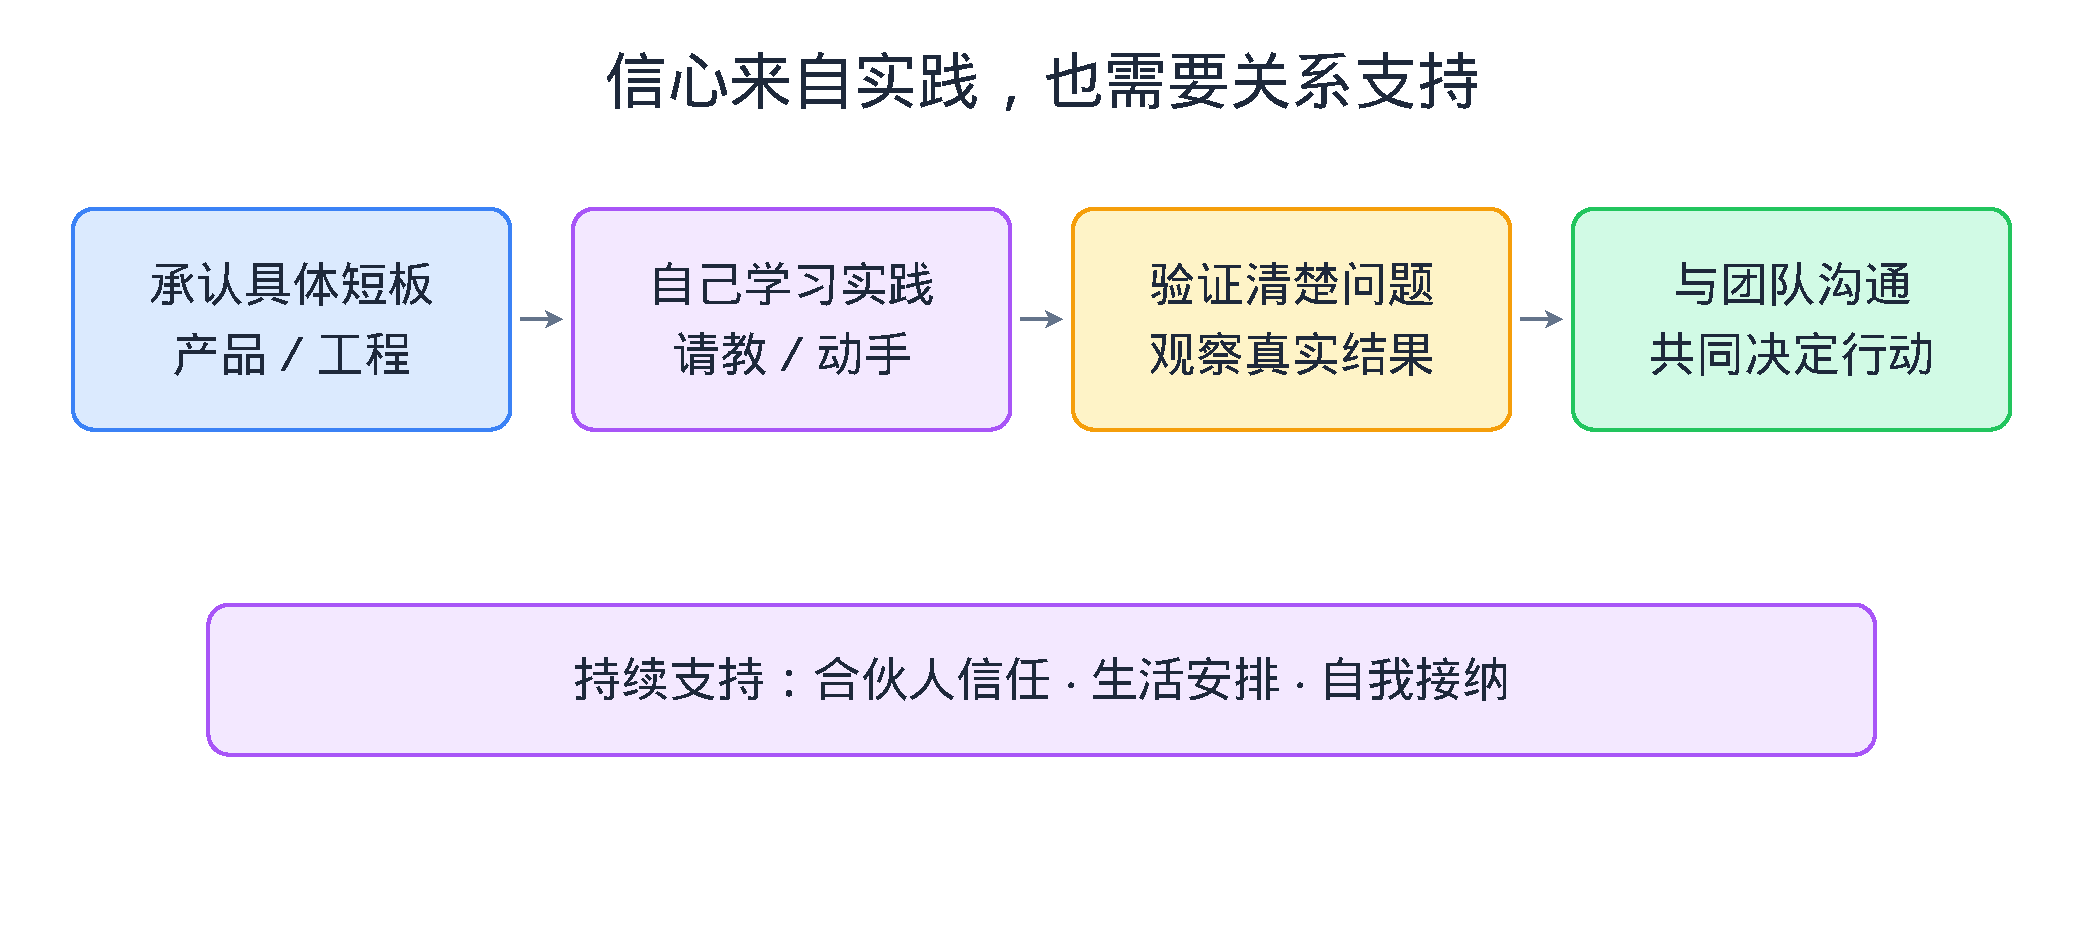
\includegraphics[width=\linewidth,height=.68\textheight,keepaspectratio]{assets/confidence-and-support.pdf}
\caption{信心来自实践，也需要关系支持；依据访谈01:07:44–01:16:00及01:41:21–01:53:44口述整理}
\end{figure}
\begin{knowledgebox}{读图：相信自己，也学会与他人一起走}
本图分为上下两层。上层从左到右由四个以实线箭头依次相连的圆角矩形组成：第一步蓝色框“承认具体短板：产品／工程”，指向第二步紫色框“自己学习实践：请教／动手”，再指向第三步黄色框“验证清楚问题：观察真实结果”，最后指向第四步绿色框“与团队沟通：共同决定行动”。下层居中放置一个宽幅紫色框，文字为“持续支持：合伙人信任 · 生活安排 · 自我接纳”。
\end{knowledgebox}
当创始人通过亲自学习与动手验证来填补能力空白、用跑通的事实与团队共同决策，并依托合伙人信任、合理生活安排与自我接纳获得持续支持时，才能在漫长的产品探索中稳步前行。
\needspace{6\baselineskip}\subsection{本章小结}
\begin{itemize}
\item \textbf{从单一标签走向整合的自我接纳}：陈春宇将支撑自己多次尝试的心力描述为从早期“比同龄人更早进实验室、发论文”的单一自我认同，转向在经历挫败与脆弱后，整合责任感、共情力与学习能力的自我接纳。
\item \textbf{靠亲自补齐短板来减少半途妥协}：复盘多次尝试的最大经验是更相信自己；遇到团队分歧或能力空白（Gap）时，不搞专断一言堂，而是通过学习产品、计算机系统与前后端开发亲自把环节跑通，再与团队共同推进。
\item \textbf{放下名校光环，在支持关系中由内向外传递力量}：认识脱离国内名校光环后的硅谷冷启动处境，珍惜相识于微末、在困难时期仍彼此信任的合伙人与投资人；从“先学会爱自己”出发，在团队协作中把事情一步步做好。
\end{itemize}
\needspace{8\baselineskip}\section{总结与延伸}
纵观陈春宇从实验室科研、初次游戏工具创业到多次AI产品迭代的历程，几条线索贯穿始终：在个人路径与归因上（第1、4章），他通过提前接触真实工作判断自身适配度，并在经历150次融资被拒与200多封冷邮件零约见后，将反思限定在具体可改进的动作上，承认时代与机遇的随机性，避免用结果倒推个人的道德优劣。在商业与工程验证上（第2、3、5章），他从错失未交割的口头意向、脱离业务场景的大厂合作及零用户的多智能体框架中吸取教训，学会用三周手写IM原型补齐工程认识，借助开源Telegram客户端测试真实使用频次，区分“可做下去的企业SaaS需求”与“自己真正想做的沟通产品”。在产品打磨与心力支撑上（第6、7章），他将跨语言语音链路（ASR—翻译—TTS）的优化建立在真实用户打分与西语裔社区、ESL课堂的实地交流之上。

访谈收尾处关于自我接纳、合伙人信任与身边关系的讨论尤为值得体会：脱离国内名校光环进入硅谷冷启动环境后，支撑团队熬过资金低谷的，是相识于微末的合伙人“陪着走完最后一程”的信任，以及创始人在挫败与脆弱中学会接纳自我、亲自补齐工程与产品短板的行动。陈春宇将“先学会爱自己”放在生活排序的起点——在稳定的支持关系中照顾好自己的状态，进而为家人、同事和股东提供更好的条件，在与团队的协作中一步步把产品做好，让身边的环境与更广泛的用户从中受益。
\subsection{拓展阅读}
以下资料供回看节目、查阅术语与继续学习。
\begin{itemize}
\item 月球大叔：本期原视频：\url{https://www.youtube.com/watch?v=jjyG9-dNZAo}
\item Intent 官方产品介绍：\url{https://intent.app/}
\end{itemize}
\end{document}
